\documentclass[a4paper]{article} 
\usepackage[intlimits,tbtags]{amsmath}
\usepackage{amssymb}   
\usepackage{amsfonts}
\usepackage{latexsym}  
\usepackage{amsxtra}   
\usepackage{amstext}   
\usepackage{bm}        
\usepackage{amsthm}    
\usepackage{amscd}     
\usepackage[dvipsnames]{xcolor}
\usepackage{marvosym}
\usepackage[utf8]{inputenc}
\usepackage[shortlabels]{enumitem}
\usepackage{array}
\usepackage{hyperref}
\usepackage{graphicx}
\usepackage[english]{babel}
\usepackage{amsmath}
\usepackage{graphicx}
\usepackage[colorinlistoftodos]{todonotes}
\newcommand{\E}{\mathbb{E}}
\newcommand{\hatt}{\hat{\theta}_m}
\usepackage{algorithm}
\usepackage{algpseudocode}
\usepackage{tikz}
\usepackage{hyperref}

\title{Summary of the Deep Learning Lecture at the University of Bonn}


\author{Tim Nogga}

\begin{document}


\maketitle
\tableofcontents
                                                                                                                                
\section{Introduction}
\subsection{Task T}
Machine Learning Tasks describes how a machine learning system learns from data. Such data can be images(pixels) among many. Typical Tasks include Klassification, Regression, and Density Function Estimation.

\subsection{Experience E}
Specifies the Information an Algorithm can use during the Learning Process.

\subsubsection{Supervised Learning}
The Algorithm is given a dataset with the correct answers. The Algorithm then tries to learn the mapping from the input to the output. This can be described with an Estimation $p_data(y|x)$.

\subsubsection{Unsupervised Learning}
The Algorithm is given a dataset without the correct answers. The Algorithm then tries to learn the underlying structure of the data. This can be described with an Estimation $p_data(x)$.

\subsection{Performance Measure P}
Learning Algorithms can be evaluated based on their Performance. In Classification Problems, the Accuracy is a common measure. %TODO: what is a mittlere logarithmische Wahrscheinlichkeits von Samples?
The Perfomance Measure is calculated on a Test Set, which is not used during the Training Process. So there a are two sets a Test Set and a Training Set. 

\subsection{Training Error, Test Error and Generalization}
Generalization is the ability of an algorithm to perform well on previously unseen data. During Training the Training Error should be reduced, but the Test Error should be reduced as well. If the Training Error is reduced but the Test Error is not, the algorithm is overfitting. Meaning the algorithm is learning the noise in the data instead of the underlying structure. But if the Test Error is not even reduced the algorithm is underfitting.

\subsection{Capacity}
Overfitting and underfitting are also dependent on the capacity of the model. Say you take a model with with a low capacity, it will underfit the data, as it is not able to learn the underlying structure. But if a model with high Capacity is used, it will just memorize the data and thus overfit, as it is not able to generalize.

\subsection{Capacity vs Error}
\begin{figure}[h]
    \centering
    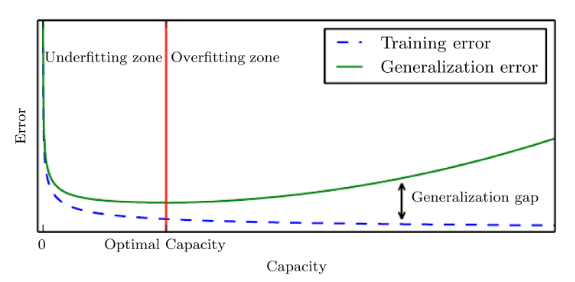
\includegraphics[width=0.8\textwidth]{images/capacity.png}
    \caption{}
    \label{fig:}
\end{figure}
It becomes apparent that the Training Error decreases with increasing Capacity. But the Test Error decreases first and then increases again. This is due to the fact that the model is overfitting the data, thus not able to generalize anymore. This is also why it is called Generalization Gap.

\subsection{Hyperparameters}
Leraning Algorithms usually have Hyperparameters which are paramters not learned during Training, but set before. These could be things such as Model Capacity and Learning Rate. This poses the Question wether Capacity Hyperparameters can be derived from the Trainingset. The answer is no, since the Learning Algorithm would always choose the highest Capacity, as it would always reduce the Training Error.

\subsection{Cross Validation}
Cross Validation can be used to determine the best Hyperparameters. The Training Set is split into k parts. Then the Algorithm is trained on k-1 parts and tested on the remaining part. This is done k times, so that every part is used as a Test Set once. The average Test Error is then used to determine the best Hyperparameters. 

\section{Recap Statistics}
\subsection{Terms and Definitions}
\begin{itemize}
    \item \textbf{Sample Space} $\Omega$: Set of all possible outcomes of an experiment. For example a dice roll has a Sample Space of $\Omega = \{1,2,3,4,5,6\}$
    \item \textbf{Event} $A$: Subset of the Sample Space. For example the Event of rolling an even number is $A = \{2,4,6\}$
    \item \textbf{Sigma Algebra} Collection of Events. For example the Sigma Algebra of the dice roll is $\sigma(\Omega) = \{\emptyset, \{1,2,3,4,5,6\}, \{1,3,5\}, \{2,4,6\}\}$
    \item \textbf{Measurable space} $(\Omega, \mathcal{A})$: Is a Measurable Space if $\Omega$ is a Sample Space and $\mathcal{A}$ is a Sigma Algebra.
\end{itemize}

\begin{itemize}
    \item \textbf{Probability Density Function if $\Omega$ is Discrete} x $p: \Omega \rightarrow [0,1]$ with $\sum_{\omega \in \Omega} p(\omega) = 1$. 
    \item \textbf{Probability Density Function if $\Omega$ is Continuous} x $p: \Omega \rightarrow [0,\infty)$ with $\int_{\omega \in \Omega} p(\omega) d\omega = 1$.
\end{itemize}

\subsection{Multivariate Statistics}
It just means that there are more than one Random Variable. For example if we have two Random Variables $X$ and $Y$ we can define a Joint Probability Density Function $p(x,y)$.

\subsection{Marginalization in a Discrete Case}
We can get the PDF of one Random Variable by summing over the other. For example $p(x) = \sum_{y} p(x,y)$. or $p(y) = \sum_{x} p(x,y)$.
In the Case of getting $p(x)$ this is just Summing over all possible values of $y$, which is rather Intuitive. 

\subsection{Marginalization in a Continuous Case}
In the Continuous Case we have to integrate over the other Random Variable. For example $p(x) = \int p(x,y) dy$. or $p(y) = \int p(x,y) dx$.

\subsection{Marginalization in a Mixed Case}
In a Mixed case if $p(x)$ is Continuous and $p(y)$ is Discrete we have to sum over $y$ and integrate over $x$. For example $p(x) = \int p(x,y) dy$ or $p(y) = \sum_{x} p(x,y)$.

\subsection{Marginalization in Multiple Dimensions}
If we for example want to know (p(x,y) given 4 parameters x,y,z,w) we have to marginalize over z and w. If w is Discrete we sum over w and if z is Continuous we integrate over z. This results in the following $p(x,y) = \sum_{w} \int p(x,y,z,w) dz dw$.

\subsection{Conditional Probability}
The Conditional Probability is defined as $p(x|y = y_1)$ and is the Probability of $x$ given that $y$ is $y_1$. 
 $p(x|y = y^{*}) = \frac{p(x,y = y^{*})}{p( y = y^{*})}$
 This is rather intuitiv aswell if you imagine that you are only interested in this one case where $y$ is $y^{*}$. And then you will need to devide by the Probability of this case happening, independent of $x$.

This can be rewritten as $p(x|y) = \frac{p(x,y)}{p(y)}$. \\
Which in turn can be rewritten as $p(x,y) = p(x|y) p(y)$ and $p(x,y) = p(y|x) p(x)$.

\subsection{Independence}
Two Random Variables are independent if $p(x,y) = p(x) p(y)$. This means that the Probability of $x$ and $y$ happening is the same as the Probability of $x$ happening times the Probability of $y$ happening.

\subsection{independent and Identically Distributed}
As an example one could think of a Dice Roll. The Dice Roll is independent and identically distributed, as the Probability of rolling a 1 is the same for every roll and the Probability of rolling a 1 and a 2 is the same as the Probability of rolling a 1 times the Probability of rolling a 2.
Formally this can be written $p(x_1, x_2, ..., x_n) = p(x_1) p(x_2) ... p(x_n).$

\subsection{Bayes Rule}
As previously discussed we have $ p(x,y) = p(x|y)p(y) and p(x,y) = p(y|x)p(x)$
By setting these two equations equal we get $p(y|x)p(x) = p(x|y)p(y)$
This can be rewritten as $p(y|x) = \frac{p(x|y)p(y)}{p(x)}$ which is the Bayes Rule.
With the backknowledge that $p(x) = \sum_{y} p(x|y)p(y)$ for discrete  and $p(x) = \int p(x|y)p(y) $ for Continuous cases  we can rewrite the Bayes Rule as $p(y|x) = \frac{p(x|y)p(y)}{\sum_{y} p(x|y)p(y)}$ or $p(y|x) = \frac{p(x|y)p(y)}{\int p(x|y)p(y) dy}$.
Here the Likelihood is the $p(x|y)$, the Prior is the $p(y)$ and the Posterior is the $p(y|x)$ and the Evidence is the $p(x)$. The Likelihood is the the Probability to observe a certain x given a certain y. The Prior is the Probability of y happening. The Posterior is the Probability of y happening given x. The Evidence is the Probability of x happening.

\subsection{Expectation}
The Expectation is the average value of a Random Variable. It is defined as $E[x] = \sum_{x} x p(x)$ for Discrete Random Variables and $E[x] = \int x p(x) dx$ for Continuous Random Variables.

\subsection{Variance and Standard Deviation}

The Variance is a measure of how much the values of a Random Variable differ from the mean. It is defined as $Var[x] = E[(x - E[x])^{2}] = E[x^{2}] - E[x]^{2}$.
The Standard Deviation is the square root of the Variance. It is defined as $\sigma = \sqrt{Var[x]}$.

\subsection{Shannon Entropy}

The Shannon Entropy gives us an answer to the Question how many bits are needed to encode Samples from a Probability Distribution. It is defined as $H(x) = - \sum_{x} p(x) \log p(x) = E[- \log(p(X))]$ for Discrete Random Variables. 
This can be used to measure the Uncertainty of a Random Variable. If the Entropy is high, the Random Variable is uncertain. If the Entropy is low, the Random Variable is more certain.
So for a Coin Flip the Entropy would be $H(x) = - \frac{1}{2} \log \frac{1}{2} - \frac{1}{2} \log \frac{1}{2} = 1$. This means that it takes 1 Bit to encode the Coin Flip. 

\subsection{Cross Entropy}

The Cross Entropy is the same as the Shannon Entropy, but for two Probability Distributions. It is defined as $H(p,q) = - \sum_{x} p(x) \log q(x) = E_p[- \log(q(X))]$ for Discrete Random Variables. This can be used to measure the difference between two Probability Distributions. If the Cross Entropy is high, the Distributions are different. If the Cross Entropy is low, the Distributions are similar.

\subsection{Kullback-Leibler Divergence}

The Kullback-Leibler Divergence is a measure of how much one Probability Distribution differs from another. It is defined as $D_{KL}(p||q) = H(p,q) - H(p) = \sum_{x} p(x) \log \frac{p(x)}{q(x)} = E_p[\log \frac{p(X)}{q(X)}]$ for Discrete Random Variables. This can be used to measure the difference between two Probability Distributions. If the Kullback-Leibler Divergence is high, the Distributions are different. If the Kullback-Leibler Divergence is low, the Distributions are similar, if the Divergence is 0 the Distributions are the same.

\section{Estimators}
\subsection{Point Estimation}

A Point Estimator is a function of the data that is used to estimate an unknown parameter $\hat{\theta}$ This can also be interpreted as an Learning Algorithm, where the Parameter is supposed to be learned. The Point Estimator is denoted as $\hat{\theta}$. 

\subsection{Bias}

The Bias of an Estimator is the difference between the expected value of the Estimator and the true value of the parameter. It is defined as $Bias(\hat{\theta}) = E[\hat{\theta}] - \theta$. If the Bias is 0, the Estimator is unbiased.

\subsection{Mean Squared Error}

The Mean Squared Error is a measure of how well an Estimator performs. This was also discussed on one of the Tasks handed out. Here we had to Prove that the Mean Squared Error can be decomposed into the Variance of the Estimator and the Bias of the Estimator. 
\begin{align*}
    \text{MSE}(\hatt) &= \text{Bias}(\hatt)^2 + \text{Var}(\hatt) \\
    \Leftrightarrow \E[(\hatt - \theta)^2] &= (\E[\hatt] - \theta)^2 + \E[\hatt^2] - \E[\hatt]^2 \\
    \Leftrightarrow \E[\hatt^2 - 2\hatt\theta + \theta^2] &= \E[\hatt]^2 - 2\E[\hatt]\theta + \theta^2 + \E[\hatt^2] - \E[\hatt]^2 \\
    \Leftrightarrow \E[\hatt^2] - 2\E[\hatt]\theta + \theta^2 &= \E[\hatt^2] - 2\E[\hatt]\theta + \theta^2
\end{align*}


The Mean Squared Error can be decomposed into the Variance of the Estimator and the Bias of the Estimator. If the Mean Squared Error is low, the Estimator is good. The Goal of an Estimator is to minimize the Mean Squared Error.

\subsection{Bias-Variance Tradeoff}
\label{sec:Bias-Variance Tradeoff}
\begin{figure}[h]
    \centering
    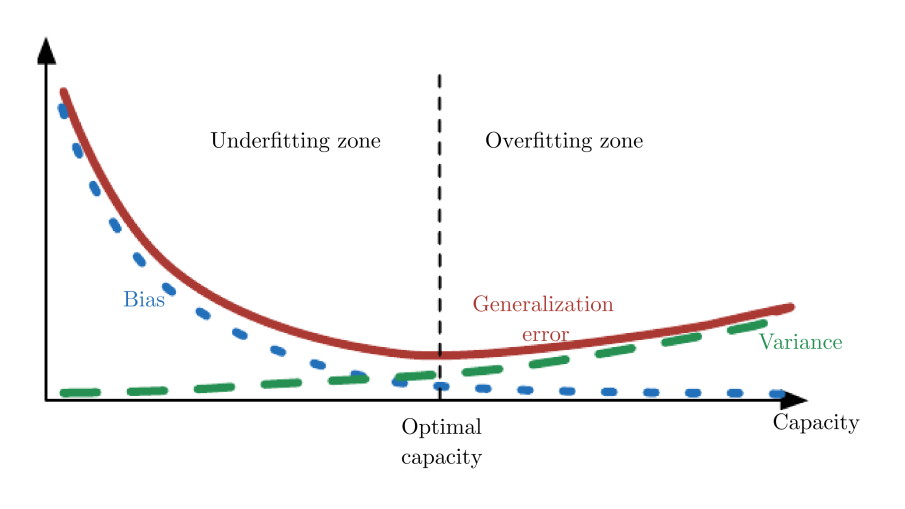
\includegraphics[width=0.8\textwidth]{images/bias_variance_tradeoff.png}
    \caption{}
    \label{fig:}
\end{figure}

As Depicted in the Figure, the Bias and the Variance are inversely proportional. If the Bias is high, the Variance is low and vice versa. The Goal is to find the sweet spot where the Bias and the Variance are both low. This is called the Bias-Variance Tradeoff.

\subsection{Point Estamation and the Consinstency of the Estimator}
A Point Estimator is consistent if it converges in Probability to the true value of the parameter. This means that the Estimator is getting better and better with more data. Formally this is written as $\lim_{m \rightarrow \infty} P(|\hat{\theta}_m - \theta| > \epsilon) = 0$. 

\subsection{Maximum Likelihood Estimation}

The Maximum Likelihood Estimation is a method to estimate the parameter previously discussed. It is defined as $\hat{\theta}_{ML} = \arg \max_{\theta} p_{model}(X|\theta) = \arg \max_{\theta} \prod_{i = 1}^{m} p_{model}(x_{i}|\theta)$. This means that the Maximum Likelihood Estimation maximizes  $ \hat{\theta}_{ML} $ given the data $X$.
With no poof what so ever we will assume, that the Maximum Likelihood Estimation is consistent, when the true distrubution $p_{data} $ is in the model class and $p_{data}$ is a Value of $\theta$ 

\subsection{(Negative) Log Likelihood}

Since it is numerically Problematic to take the Product, due to overflow/underflow we can take the Logarithm of the Likelihood. This is called the Log Likelihood. It is defined as 

\begin{align*}
    \arg\max_{\theta} \log p_{model}(X|\theta) &= \arg\max_{\theta} \log \prod_{i = 1}^{m} p_{model}(x_{i}|\theta) \\
    &= \arg\max_{\theta} \sum_{i = 1}^{m} \log p_{model}(x_{i}|\theta) \\
    \arg\min_{\theta} \left(- \log p_{model}(X|\theta)\right) &= \arg\min_{\theta} \left(- \sum_{i = 1}^{m} \log p_{model}(x_{i}|\theta)\right)
\end{align*}
The last Equation is the Negative Log Likelihood. It is the same as the Log Likelihood, but with a minus sign in front. This is done to make it a minimization Problem, as most Optimization Algorithms are designed to minimize a Function.

\subsection{Negative Log-Likelihood and Cross Entropy}
Negative Log-Likelihood and Cross Entropy are equivalent when m approaches infinity. This is due to the fact that the Negative Log-Likelihood is the average Cross Entropy. This can be shown as follows:
Given that the samples \( x_i \) are drawn from the true data-generating distribution \( p_{data}(x) \), and the negative log-likelihood (NLL) is divided by the number of samples \( m \), the expression for \( m \to \infty \) approximates the cross-entropy between the modeled distribution \( p_{model}(x|\theta) \) and the true data-generating distribution \( p_{data}(x) \):

\begin{align*}
    \frac{1}{m} \sum_{i=1}^{m} - \log p_{model}(x_i|\theta) &\approx \mathbb{E}_{x \sim p_{data}}[-\log p_{model}(x|\theta)] \\
    &= -\int p_{data}(x) \log p_{model}(x|\theta) \, dx \\
    &\approx H(p_{data}, p_{model})
\end{align*}

As \( m \to \infty \), the average NLL converges to the cross-entropy between \( p_{data} \) and \( p_{model} \).

\subsection{Conditional Negative Log-Likelihood}
We can generalize the Negative Log-Likelihood to the Conditional Negative Log-Likelihood. This is done by conditioning the Negative Log-Likelihood on the input. It is defined as $\arg \min_{\theta} \sum_{i = 1}^{m} - \log p_{model}(y_{i}|x_{i}, \theta)$. This is particularly useful, because it can be used in Classification, Segmentation, among many other Tasks, where we want to Intepret the conditional Probability of the output given the input.

\subsection{Cross Entropy for Classification/Segmentation}
In Classification and Segmentation Problems a Neural Network usually learns Probability Function right away lets call it $p_{\theta}(y|x)$ This leads to the following Negative Log Likelihood: $- \log p(Y|X,\theta) =  \sum_{i} - \log p(y_{i}|x_{i}, \theta)$.  
Thus follows the Cross Entropy Loss: $H = \frac{1}{m} \sum_{i} - \log p_{\theta}(y_{i}|x_{i})$
\subsection{Segmentation and Pixel Wise Classification}
In Segmentation and Pixel Wise Classification the Cross Entropy Loss is calculated for every Pixel. This is done by calculating the Cross Entropy Loss for every Pixel and then averaging over all Pixels. This is done to get a single Value for the Loss.
\begin{figure}[h]
    \centering
    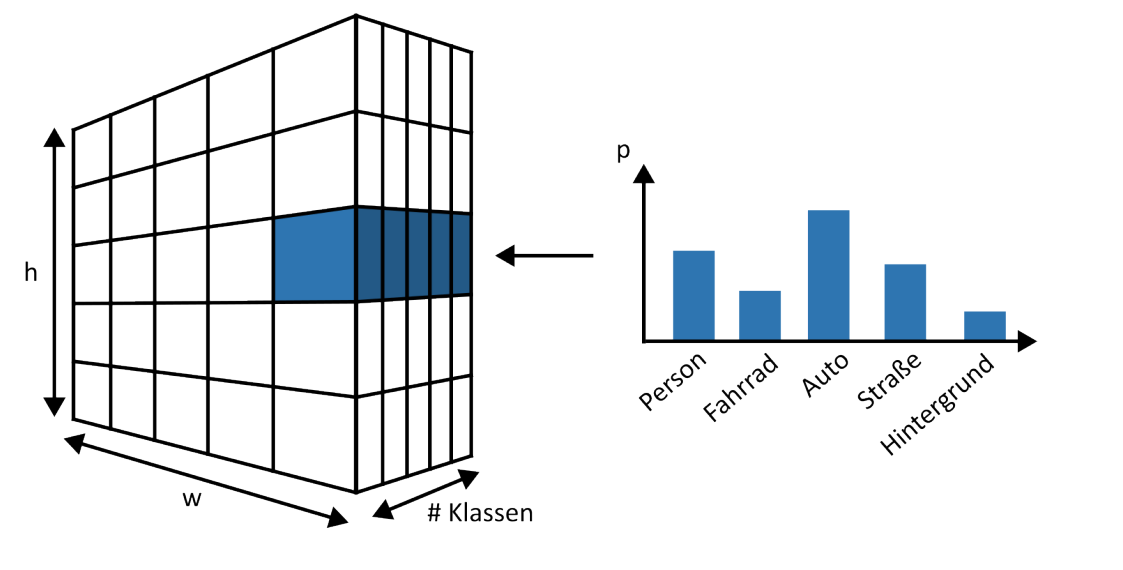
\includegraphics[width=0.8\textwidth]{images/pixel_wise.png}
    \caption{}
    \label{fig:}
\end{figure}
The Figure is a visualization of the Cross Entropy Loss for a Pixel Wise Classification Task. Every Layer here represents a Class. So here the average for all Classes is calculated and then compared to get a Classification Result. 

\subsection{Mean Squared Error for Regression}
If we consider the Normal Distribution as the Model Distribution, the mean of that is learned by the Neural Networks, considering most Regression Problems. This leads to the Likelihood being defined as $p(Y|X,\theta, \sigma) = \prod_{i} \mathcal{N}(y_{i},\mu_{\theta}(x_{i}),\sigma)$
Thus follows the Negative Log Likelihood: $- \log p(Y|X,\theta, \sigma) =  \sum_{i} \frac{1}{2} 2(\pi \sigma^{2}) + \frac{1}{2} \frac{(y_{i} - \mu_{i}(x_{i}))^{2}}{\sigma^{2}}$. If we assume that the Variance is constant, we can drop the first term, also the Denominator can be dropped, as it is constant aswell. This leads to the Mean Squared Error: $MSE = \frac{1}{m} \sum_{i} (y_{i} - \mu_{i}(x_{i}))^{2}$
The minimum of the Mean Squared Error is if $\mu(x_{i}$ is the mean of the samples.)


\subsection{Mean Absolute Error}
For the MAE or $L{1}$ a Laplace Distribution is assumed. This leads to the Likelihood being defined as $p(Y|X,\theta, \sigma) = \prod_{i} \mathcal{L}(y_{i},\mu_{\theta}(x_{i}),\sigma)$ With the NLL being defined as $- \log p(Y|X,\theta, \sigma) =  \sum_{i} log(2 \sigma) + \frac{|y_{i} - \mu_{i}(x_{i})|}{\sigma}$. This leads to the Mean Absolute Error: $MAE = \frac{1}{m} \sum_{i} |y_{i} - \mu_{i}(x_{i})|$ The Major difference is the missing squared making it more robust to outliers. But also the minimum is not the mean of the samples, but the median. 

\subsection{Maximum A Posteriori Estimation}
An alternative to the Maximum Likelihood Estimation is the Maximum A Posteriori Estimation. It is defined as $\hat{Theta}_{MAP} = \arg \max _{\theta} p(\theta|X)$
Assuming $\theta$ is a random variable, we can use Bayes Rule to rewrite this as $\hat{\theta}_{MAP} = \arg \max _{\theta} p(X|\theta) p(\theta)$ To further simplify the operations, we can take the log as per usual. This leads to $\hat{\theta}_{MAP} = \arg \max _{\theta} \log p(X|\theta) + \log p(\theta)$ Here we can incoperate a sum again thus follows $\hat{\theta}_{MAP} = \arg \max _{\theta} \sum_{i} \log p(x_{i}|\theta) + \log p(\theta)$
The is as the Name already hints, the Maximum Likelihood Estimation with a Prior. This is useful if we have some prior knowledge about the parameter. With backround knowledge we can push $\theta$ to a realistic value. Say we have knowledge X we can have  $P(Y|X,\theta)$ here the same with x follows $\hat{\theta}_{MAP} = \arg \max _{\theta} \sum_{i} \log p(x_{i}|x_{i}\theta) + \log p(\theta)$
This is a key Concept later on for Regularization of Weights for Neural Networks.

\section{Error functions}
The NLL  $\hat{\theta}_{ML} =  \arg\min_{\theta} (- \sum_{i = 1}^{m} \log p(x_{i}|\theta)) = \arg \min_{\theta} f(\theta)$ the Maximum Likelihood Estimator will now be viewed as the minimum of a Function. One might notice that this does not look too different from minimizing or maximizing a function during Training in Machine-Learning. This would in that Context be reffered to as  Objective Function, cost function, error function or loss function. The Variable $\theta$ that is to be Optimized would then be equivalent to the Parameters of the Model. Thus the Maximum Likelihood Point Estimation is equivalent to a Machine Learning Algorithm. 
The obvious question now is, how do we minimize this function?



\subsection{Local and Global Minima}
\begin{figure}[h]
    \centering
    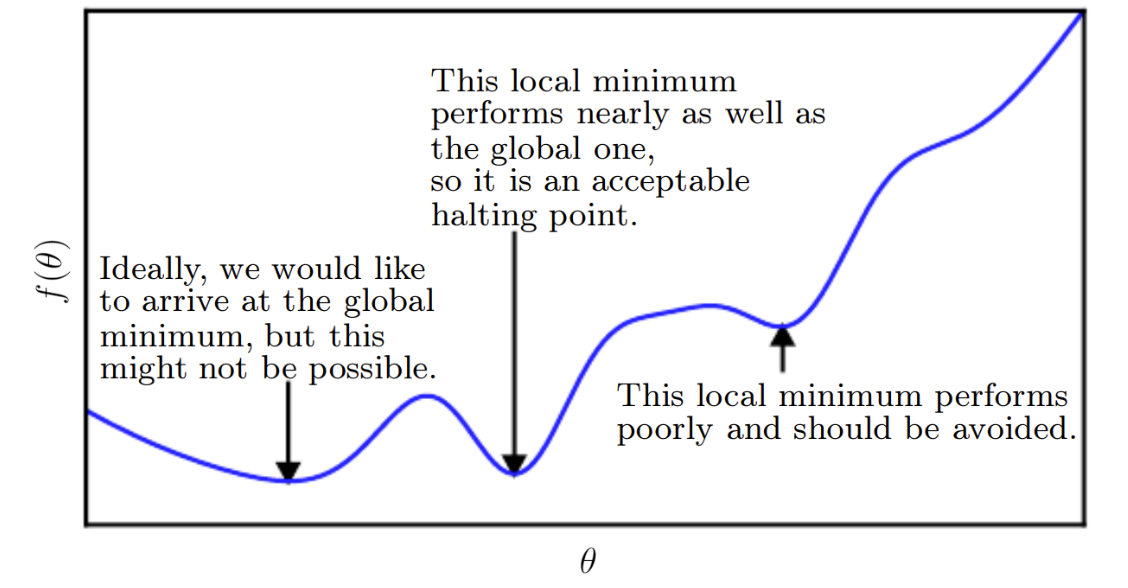
\includegraphics[width=0.8\textwidth]{images/local_global.png}
    \caption{}
    \label{fig:Local vs Global Minima}
\end{figure}
As explained before the Local Minima is the one found by Gradient Descent. This might not be too bad if it is approximitely the same as the Global Minima. But if it is not, the Algorithm will get stuck in the Local Minima. A good rule of thumb is to compare the Local Minima to low values of the cost function, if they are not far off, the Local Minima is good enough.

\newpage
\subsection{Convex Functions}
Convex function if $\forall x,y \in D  \text{and} t \in [0,1] \rightarrow f(tx + (1-t)y) \leq tf(x) + (1-t)f(y)$ hold. This basically just means that every point is below the average of the two points. Convex Functions have the nice property that they have only one minimum. However this is rather rare in the context of Machine Learning.


\begin{figure}[h]
    \centering
    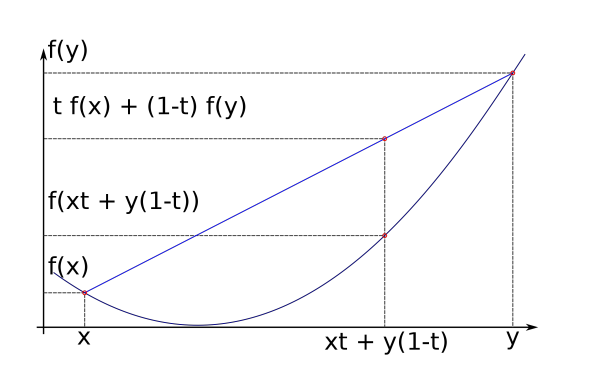
\includegraphics[width=0.8\textwidth]{images/convex.png}
    \caption{}
    \label{fig: Illustration of Convexity}
\end{figure}

\subsection{Different approaches to find Minima}

\subsubsection{Least Squares}
Least Squares is a method to find $\hat{\theta}$ for a linear Model this is done by taking $\arg \min_{\theta} ||A \theta - y ||^{2} = (A^{*}A)^{-1} A^{*}y$ This only works for least squares though and Machine Learning Models are usually not linear.

\subsubsection{Grid Search}
Grid Search is a method to find the minimum of a function. It is done by evaluating the function at every point on a grid. This is rather slow, as the number of points grows exponentially with the number of dimensions.

\subsubsection{Evoluationary Algorithms}
Evolutionary Algorithms are a class of algorithms that are inspired by the process of natural selection. They work by creating a population of solutions and then using genetic operators such as mutation and crossover to evolve the population over time. This is rather slow aswell, as it is a brute force method. It works fine for 10-1000 Parameters but becomes inneficient for more. It can be usefull for HyperParameters though. 

\subsubsection{Gradient Based Optimization}
If the Model and the Error Function are differentiable, Gradient Based Optimization can be used. This is done by calculating the Gradient of the Error Function and then following the Gradient to the minimum.

\section{Gradient Descent}
\subsection{Error Surface}

\begin{figure}[h]
    \centering
    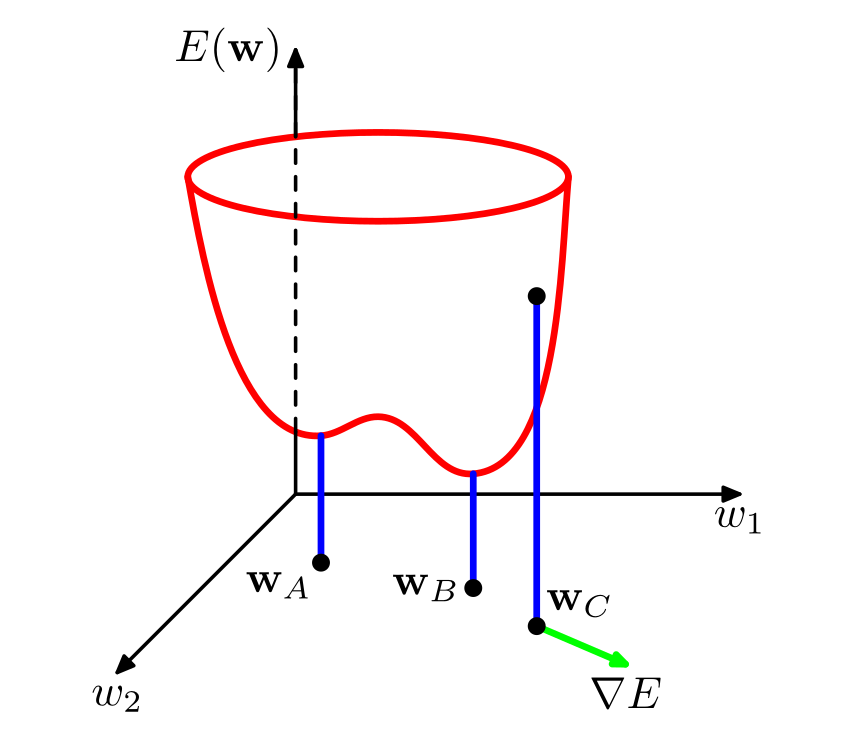
\includegraphics[width=0.8\textwidth]{images/error_surface.png}
    \caption{}
    \label{fig:Error Surface}
\end{figure}

This is a Geometric Representation of the Errror Function. $w_{A} , w_{B}$ is a local and a Global minimum. Here Gradient Descent comes in handy. If we start at a random point, here $w_{C}$ we can follow the Gradient to the minimum. So basically we just find the derivative of the function, follow the Gradient to the opposite direction and repeat this until we reach the minimum. The opposite direction is taken, as the Gradient points to the steepest ascent, and for minimization we want to go in the opposite direction.

\subsection{Formal Definition of Gradient Descent}
We are looking for $\theta$ that minimizes the Error Function $f(\theta)$ Since we can not do this analytically we will use a numerical method.  For that we choose a starting value $\theta_{0}$ and then update it iteratively. The update rule is defined as $\theta_{i+1} = \theta_{i} + \Delta \theta_{i}$ 
The usual way to do this is to introduce a learning rate $\epsilon$ and then update the parameter as follows $\theta_{i+1} = \theta_{i} - \epsilon \nabla f(\theta_{i})$

\subsection{Gradient - Taking the Derivative in Multiple Dimensions}
The Error Function of a Neural Net is usually dependent on multiple Parameters. This is why it becomes necessary to talk about partial derivatives, thus the concept of Gradients is introduced. Let $f(\theta)$ be a skalar Function. Meaning it mapps from $\mathbb{R}^{n} \rightarrow \mathbb{R}$. The Gradient of $f$ is defined as $\nabla f(\theta)_{i} = \frac{\partial f(\theta)}{\partial \theta_{i}} f(\theta)$ This is just the partial derivative of $f$ with respect to $\theta_{i}$. If u write this in vector form it becomes $\nabla f(\theta) = \begin{pmatrix} \frac{\partial f(\theta)}{\partial \theta_{1}} \\ \frac{\partial f(\theta)}{\partial \theta_{2}} \\ \vdots \\ \frac{\partial f(\theta)}{\partial \theta_{n}} \end{pmatrix}$ So every entry of the Gradient is the partial derivative of $f$ with respect to the corresponding parameter in our cases usually the weight.
A stationary point is given if every entry of the Gradient is 0.

\subsection{Direcional Derivative}
The Directional Derivative describes the rate in which a function changes in a certain direction. It is defined as $\nabla_{u} f(\theta) = \lim_{\alpha \rightarrow 0} \frac{f(\theta + \alpha u) - f(\theta)}{h}$ This is just the derivative of $f$ in the direction of $u$. This can be rewritten as $\nabla_{u} f(\theta) = \nabla f(\theta) u^{T}$ This is just the dot product of the Gradient and the direction.
To minimize f, we must find the direction u, where f decreases the fastest, this means $min_{u,u^{T}u =1} \ u^{T} \nabla f(\theta) = min_{u,u^{T}u =1} ||u||_{2} \cdot ||\nabla f(\theta)||_{2} \cdot \cos(\phi) $.
where $\phi$ is the angle between the Gradient and the direction. Since u is a unit vector, the minimum can be simplified to $min_{u} \cos(\phi)$, since the Gradient is independent of u. This is due to the fact that $\cos$ oxcilates between -1 and 1. Thus the minimun is -1 and $\cos(\pi) = -1$ 

\subsection{Learning Rate $\epsilon$}
For now we will have  just take $\epsilon$ as a small constant. The danger when $\epsilon$ is too large is that may not converge to the minimum. If $\epsilon$ is too small, the convergence will be slow. This is why it is important to choose $\epsilon$ wisely.

\subsection{Jacobi Matrix}
If we now have vectors as inputs and outputs it is handy to define a Matrix called Jacobi-Matrix. This matrix conatins the partial derivative of f at the position x. It is defined as \[ (J_{f}(\theta))_{i,j} = \frac{\partial}{\partial \theta_{j}} f(\theta)_{i} \]
This can be written in the following Matrix Form \[ J_{f}(\theta) = \begin{pmatrix} \frac{\partial f_{1}(\theta)}{\partial \theta_{1}} & \frac{\partial f_{1}(\theta)}{\partial \theta_{2}} & \cdots & \frac{\partial f_{1}(\theta)}{\partial \theta_{n}} \\ \frac{\partial f_{2}(\theta)}{\partial \theta_{1}} & \frac{\partial f_{2}(\theta)}{\partial \theta_{2}} & \cdots & \frac{\partial f_{2}(\theta)}{\partial \theta_{n}} \\ \vdots & \vdots & \ddots & \vdots \\ \frac{\partial f_{m}(\theta)}{\partial \theta_{1}} & \frac{\partial f_{m}(\theta)}{\partial \theta_{2}} & \cdots & \frac{\partial f_{m}(\theta)}{\partial \theta_{n}} \end{pmatrix} \]

\subsection{The Derivative of second order}
The derivative of second order is important for us as well since it can imply the improvement that is expected of one iteration of the Gradient Descent. 

\subsection{Hessian Matrix}
The Hessian Matrix is the Matrix of second order partial derivatives of a function. It is defined as \[ H_{f}(\theta)_{i,j} = \frac{\partial^{2}}{\partial \theta_{i} \partial \theta_{j}} f(\theta) \] The directional Derivative of second order to a Directionvector u 
is given by $u^{T} H_{f}(\theta) u$. If u is an Eigenvektor of H, then the derivative of second order is equivalent to the corresponding Eigenvalue. For other directions, the derivative of second order is the weighted average of the Eigenvalues.
Where Directions which correspond better with the Eigenvalues are more important. This also implies that the second directional derivative is beween the smallest and the largest Eigenvalue of H, because it is a weighted sum, it must be contrained by the smallest and the largest Eigenvalue.

This is also equivalent to the Jacobi Matrix of the Gradient. 

\subsection{Approximate Second-Order Methods}
Let's have a look at the Newton Method. The Newton Method is used to find the minimum of a function. It is defined as $\theta_{i+1} = \theta_{i} - H_{f}(\theta_{i})^{-1} \nabla f(\theta_{i})$ This is just the Gradient Descent with the Hessian Matrix. 
I mean it makes sense though, since we basically exchanged our shitty $\epsilon$ to a more dynamic way of choosing the learning rate. 
It brings some disatvantages though, as the Hessian Matrix calculation as well as the inversion can be rather expensive for large disatvantages. 

\section{Stochastic Gradient Descent}
If the calculation of the Gradient is done for the entire Dataset, it might be slow, due to the immense size. Also the data during an iteration is saved in RAM or Graphicsmemory, this can be become impossible to handle for large Datasets. This is why we introduce Stochastic Gradient Descent. Which takes Batches of the Data and calculates the Gradient for these Batches. 
Lets assume that the Trainingsample is i.i.d. then the log likelihood can be written as $L_{\theta}(X) = \frac{1}{n} \sum_{i=1}^{n} L(f_{\theta}(x_{i}),y_{i})$ which implicates that the Gradient can be written as $\nabla_{\theta} L_{\theta}(X) = \frac{1}{n} \sum_{i=1}^{n} \nabla_{\theta} L(f_{\theta}(x_{i}),y_{i})$ This is just the average of the Gradients of the Batches. 

\subsection{Mini-Batch Gradient as an unbiased Estimator}
The Approximation of the Gradient with the help of Mini-Batches can be seen as an unbiased Estimator of the Gradient. In math language we can write 
\begin{align*}
    \mathbb{E} \left[ \nabla_{\theta} L_{\theta} (\hat{X}) \right] 
    &= \mathbb{E} \left[ \frac{1}{k} \sum_{x \in \hat{X}} \nabla_{\theta} L_{\theta} (x) \right] \\
    &= \frac{1}{|\mathcal{X}_k|} \sum_{\hat{X} \in \mathcal{X}_k} \frac{1}{k} \sum_{x \in \hat{X}} \nabla_{\theta} L_{\theta} (x) \\
    &= \frac{1}{k} \sum_{x \in X} \frac{\binom{n-1}{k-1}}{\binom{n}{k}} \nabla_{\theta} L_{\theta} (x) \\
    &= \frac{1}{k} \sum_{x \in X} \frac{k}{n} \nabla_{\theta} L_{\theta} (x) \\
    &= \frac{1}{n} \sum_{x \in X} \nabla_{\theta} L_{\theta} (x) \\
    &= \nabla_{\theta} L_{\theta} (X)
    \end{align*}
    The given equations demonstrate that the expected gradient of the loss function, when computed over a randomly sampled subset of the data, equals the gradient of the loss function over the entire dataset. This result shows that using mini-batches in stochastic gradient descent  provides an unbiased estimate of the full gradient. As a result, SGD can efficiently and effectively optimize the model parameters by using only small subsets of data at each iteration, making it scalable and practical for large datasets.
    (rewritten by chatgpt so it becomes more coherent lol)


\subsection{Batch Size}
The Batch size is as per usual a trade off, either we choose large Batches. This would lead to a more accurate Gradient, but needs to more computation power. If we choose small Batches, the Gradient is less accurate, but the computation is faster. This makes it necessary to choose a smaller learning rate so the training remains stable.
For the Varianz of the Gradient $Var(\frac{1}{|I|} \sum_{i\in I} g_{i}) = \frac{1}{|I|^{2}}\sum_{i\in I}Var(g_{i})= \frac{\sigma^{2}}{|I|}$
I is a set of indices of the Patch and the Gradients are $g_{i}$ This makes sense as it exactly depicts the relation we established before the equation.
The choice of the Batch size, since it is a Tradeoff depends on several Factors
\begin{enumerate}
    \item If the Batches are processed in parallel, the Batch size should be chosen to fit the memory of the GPU.
    \item Multiprozessor Systems can't be used to their full potential if the Batch size is too small. Since the Batches have fixed cost for the computation at a certain size. 
    \item Hardware is optimized for certain Batch sizes. For GPUs this is usually $2^{n}$.
    \item Small Batches have a Regularization effect, as the Gradient is more noisy.
\end{enumerate}

\subsection{Algorithm for Stochastic Gradient Descent}
\begin{algorithm}[h]
    \caption{Stochastic gradient descent (SGD) update at training iteration $k$}
    \begin{algorithmic}
    \Require Learning rate $\epsilon_k$
    \Require Initial parameter $\theta$
    \While{stopping criterion not met}
        \State Sample a minibatch of $m$ examples from the training set $\{ x^{(1)}, \ldots, x^{(m)} \}$ with corresponding targets $y^{(i)}$
        \State Compute gradient estimate: $\hat{g} \leftarrow \frac{1}{m} \nabla_\theta \sum_{i} L(f(x^{(i)}; \theta), y^{(i)})$
        \State Apply update: $\theta \leftarrow \theta - \epsilon \hat{g}$
    \EndWhile
    \end{algorithmic}
    \end{algorithm}
    Lets go through the Algorithm step by step. First we give a learning rate and an initial parameter. Then we sample a minibatch of m examples from the training set. We compute the gradient estimate by taking the average of the gradients of the loss function over the minibatch. We then apply the update rule to the parameter by subtracting the learning rate times the gradient estimate. We repeat this process until a stopping criterion is met, which could be a maximum number of iterations, a convergence criterion, or another condition.

    \subsection{Learning Rate $\epsilon$}
    The first Parameter was the Learning Rate $\epsilon$. The Learning Rate needs to go to Infinity, so $\sum_{k=1}^{\infty} \epsilon_{k} = \infty$ and $\sum_{k=1}^{\infty} \epsilon = \infty$ Usually the learning rate is being reduced over time. This is done by a learning rate schedule. For example a linear decay, where the learning rate is reduced by a contant factor until it reaches a certain iteration, where is remains constant. 

    \subsection{Momentum}
    \subsection{Algorithm for Stochastic Gradient Descent with Momentum}
    Momentum is a method to accelerate the convergence of Gradient Descent. Momentum aggregates the Gradients of previous Iterations. $$v \leftarrow \alpha v + \epsilon \nabla_{\theta}(\frac{1}{m} \sum_{i=1}^{m} L(f(\theta^{(i)};\theta),y^{(i)})) $$ This is just the Gradient Descent with the addition of the Momentum. The Momentum is a Hyperparameter and is usually set to 0.9, 0.99, or 0.5. The Momentum is then used to update the parameter as follows $\theta \leftarrow \theta + v$ This is just the Gradient Descent with the addition of the Momentum. The Momentum is a Hyperparameter and is usually set to 0.9, 0.99, or 0.5. The Momentum is then used to update the parameter as follows $\theta \leftarrow \theta - v$
    \begin{algorithm}
\caption{Stochastic gradient descent (SGD) with momentum}
\begin{algorithmic}
\Require Learning rate $\epsilon$, momentum parameter $\alpha$
\Require Initial parameter $\theta$, initial velocity $v$
\While{stopping criterion not met}
    \State Sample a minibatch of $m$ examples from the training set $\{ x^{(1)}, \ldots, x^{(m)} \}$ with corresponding targets $y^{(i)}$
    \State Compute gradient estimate: $g \leftarrow \frac{1}{m} \nabla_\theta \sum_i L(f(x^{(i)}; \theta), y^{(i)})$
    \State Compute velocity update: $v \leftarrow \alpha v - \epsilon g$
    \State Apply update: $\theta \leftarrow \theta + v$
\EndWhile
\end{algorithmic}
\end{algorithm}
\section{Adaptive Learning Rates}
This basically just means that we can adapt the learning rate to the Parameters. There are several methods to do this. 
\begin{enumerate}
    \item AdaGrad scales a learning rate by the inverse of the square root of the sum of all historical squared gradients. This means that the learning rate is reduced for parameters that have received large gradients in the past.
    \item RMSProp is similar to AdaGrad, but uses a moving average of squared gradients instead of the sum of squared gradients. This allows the learning rate to adapt more quickly to changes in the gradients.
    \item Adam combines the ideas of momentum and RMSProp. It uses a moving average of gradients and a moving average of squared gradients to adapt the learning rate for each parameter. 
\end{enumerate}
\subsection{AdaGrad Algorithm}
\begin{algorithm}
    \caption{The AdaGrad algorithm}
    \begin{algorithmic}
    \Require Global learning rate $\epsilon$
    \Require Initial parameter $\theta$
    \Require Small constant $\delta$, perhaps $10^{-7}$, for numerical stability
    \State Initialize gradient accumulation variable $r = 0$
    \While{stopping criterion not met}
        \State Sample a minibatch of $m$ examples from the training set $\{ x^{(1)}, \ldots, x^{(m)} \}$ with corresponding targets $y^{(i)}$
        \State Compute gradient: $g \leftarrow \frac{1}{m} \nabla_\theta \sum_i L(f(x^{(i)}; \theta), y^{(i)})$
        \State Accumulate squared gradient: $r \leftarrow r + g \odot g$
        \State Compute update: $\Delta \theta \leftarrow -\frac{\epsilon}{\delta + \sqrt{r}} \odot g$ \hspace{0.2cm} (Division and square root applied element-wise)
        \State Apply update: $\theta \leftarrow \theta + \Delta \theta$
    \EndWhile
    \end{algorithmic}
    \end{algorithm}
    So the steps added here are the Accumulation of the squared Gradient, and the update. As mentioned in the short description before, since the Multiplikation and the Division are applied element wise, the update is done for every parameter and so every parameter that was previosuly large will have a reduced learning rate. The other algorithms for other adaptive learning rates are similar to this one, but with the steps I descibed before.
    \section{Feed-Forward Networks}

    \subsection{Single-Neuron}

    The output of  single Neuron with D input values $x_{i}$, weights $w_{i}$ and Bias b can be calculated as follows: $$a = \sigma(\sum_{i=1}^{D} w_{i}x_{i} + b)$$ where $\sigma$ is the activation function. The activation function is usually a non-linear function, such as the sigmoid function, the tanh function, or the ReLU function. The output of the neuron is then passed through the activation function to produce a non linear output. This is done, so that the Model can learn non-linear relationships between the input and the output, otherwise the Model would just be a linear regression.

    \subsection{One Layer and multiple Neurons}
    Often a layer is defined by Multiple Neruons, those are fed with the same input and combined in one layer. The output of such a layer can be calculated by $$a = \sigma(\sum_{i=1}^{D}w_{ji} \cdot x_{i} + b_{j})$$ The Compact form of this would be $a = \sigma(Wx + b)$ where $W$ is the Matrix of the weights and $b$ is the Bias.


    \subsection{Multiple Layers}

    Well, now that we have the definition of one Layer down, why not do Multiple and thus create a neural Net. The output of a Neural Net with L layers can be calculated as follows: \begin{align*}
        a^{(1)} &= \sigma(W^{(1)}x + b^{(1)}) \\
        a^{(2)} &= \sigma(W^{(2)}a^{(1)} + b^{(2)}) \\
        &\vdots \\
        a^{(L)} &= f^{out} (W^{(L)}a^{(L-1)} + b^{(L)})
    \end{align*}
    Now we can consider writing this as a parameterized function
  
    \[
\text{nn}_{\theta}(x) = f_{\text{out}} \left( W^{(N)} \cdot f^{(N-1)} \left( \ldots W^{(2)} \cdot f^{(1)} \left( W^{(1)} \cdot x + b^{(1)} \right) + b^{(2)} \ldots \right) + b^{(N)} \right)
\]

With the parameters:

\[
\theta = \left( (W^{(1)}, b^{(1)}), (W^{(2)}, b^{(2)}), \ldots, (W^{(N)}, b^{(N)}) \right)
\]
The f I use is just a placeholder for the activation function.

How many layers exist is something we will define with the amount of layers being the amount of weight matrices used for Multiplication. 

\subsection{Fun Facts for Linear Activation}
Lets say we decide to use a linear function, lets show by its properties that it is not a good choice. 

\[
\text{nn}_{\theta}(x) = f_{\text{out}}\left(W^{(N)} \cdot f^{(N-1)}\left(\cdots f^{(2)}\left(W^{(2)} \cdot f^{(1)}\left(W^{(1)} \cdot x\right)\right)\right)\right)
\]

This can be simplified by grouping the weight matrices and activation functions:

\[
\text{nn}_{\theta}(x) = f_{\text{out}}\left(W^{(N)} \cdot f^{(N-1)}\left(\cdots f^{(2)}\left(W^{(2)} \cdot W^{(1)} \cdot f^{(1)}(x)\right)\right)\right)
\]

Combining weights into a single matrix \(W'\):

\[
\text{nn}_{\theta}(x) = f_{\text{out}}\left(W^{(N)} \cdots W^{(2)} \cdot W^{(1)} \cdot f^{(N-1)} \circ f^{(2)} \circ f^{(1)}(x)\right)
\]

Finally, we get:

\[
\text{nn}_{\theta}(x) = f_{\text{out}}\left(W' g(x)\right)
\]

\subsection{Activation Functions}
The Activation Function is a non-linear function that is applied to the output of a neuron. As shown before we do need those non-linear Activation Functions to learn non-linear relationships. We can differentiate beween two Sorts of here, one being for Hidden Layers (So the Layers between the Input and the Output) 
and the other for the Output Layer. Some of the Hidden Layer Activation Functions are:
\begin{itemize}
    \item Sigmoid: $\sigma(x) = \frac{1}{1 + e^{-x}}$
    \item Tanh: $\tanh(x) = \frac{e^{x} - e^{-x}}{e^{x} + e^{-x}}$
    \item ReLU: $ReLU(x) = \max(0,x)$
    \item Hard Tanh: $HardTanh(x) = \max(-1, \min(1,x))$
    \item Softplus: $Softplus(x) = \log(1 + e^{x})$
    \item 
\end{itemize}
Some of the Output Layer Activation Functions are:
\begin{itemize}
    \item Linear: $f(x) = x$
    \item Sigmoid: $\sigma(x) = \frac{1}{1 + e^{-x}}$
    \item Softmax: $Softmax(x) = \frac{e^{x_{i}}}{\sum_{j} e^{x_{j}}}$
\end{itemize}
For the output Functions it is maybe important to note that you can use the Sigmoid Function for Binary Classification and the Softmax Function for Multiclass Classification. 

\subsection{Symmetries in Parameter Space}
There are many ways to achieve the same mapping of input to output values, even though the weight matrices and biases are different. One way is to permute the neurons in a layer, this leads to $M!$ equivalent solutions. Some activation functions are also point reflections, meaning that $f(x) = f(-x)$, this leads to $2^{M}$ equivalent solutions. 
An Example for this would be $tanh(-x) = -tanh(x)$ If we combine those symmetries, we get $2^{M} \cdot M!$ equivalent solutions. This also there are as many equivalent local Minima. Which is ok though, as large networks local Minimas are usually quite good. 

\subsection{Universal Approximation Theorem}
This Theorem  states that if we have 2 layers, with enough hidden units, 
we can approximate any Continuous Function.

\section{Backpropagation}
\subsection{Why do we need Backpropagation?}
 As discussed in Chapter 5 we use gradient descent to minimize the error function. The error function is a function of the parameters of the model, and we need to compute the gradient of the error function with respect to the parameters in order to update them. 
 Perhaps a rather simple approach would be to to calculate the Difference quotient being defined by $$\frac{\partial L}{\partial W_{ji}} = \frac{L(W_{ji} + \epsilon) - L(W_{ji} - \epsilon)}{2 \epsilon} + \underbrace{O(\epsilon^{2})}_{residual \ corrections}$$ This is a rather simple approach, but it is not very efficient, since you need to evaluate the Loss-Function twice for every Parameter. As this is why we use the Backpropagation Algorithm.

 \subsection{Lets look at the Chain Rule}
 For Backpropagation we first need to understand the chain rule. The chain rule in 1D is defined as $(g \circ f)' (x) = g' (f(x)) \cdot f'(x)$. This is also written as $\frac{x}{\partial x} g(f(x)) = \frac{\partial g}{\partial f} \frac{\partial f}{\partial x}$.
 If our function depends on multiple variables, for example $x$ and $y$ then we can look at the partial derivatives. Meaning the partial derivative of $f(x,y) $ with respect to $x$ can be written as $\frac{\partial f}{\partial x}$. And with respect to $y$ as $\frac{\partial f}{\partial y}$. 

 \newpage
 \subsection{Direcional Derivative with the Chain Rule}
 \begin{figure}[h]
    \centering
    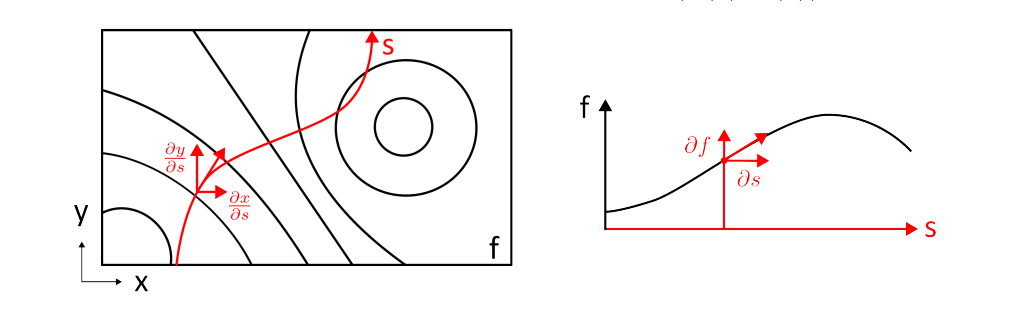
\includegraphics[width=0.8\textwidth]{images/richtungsableitung.png}
    \caption{}
    \label{fig:Richtungsableitung}
\end{figure}
Ok lets say our goal is to calculate the partial derivative of f to s, on the left graph.  Well to analyze we take the chain rule, meaning we can express $f$ as $f(x(s),y(s))$ and can then write the partial derivative of $f$ with respect to $s$ so $\frac{\partial f}{\partial s} = \frac{\partial f}{x} \frac{\partial x}{\partial s} + \frac{\partial f}{\partial y} \frac{\partial y}{\partial s}$. This is just the chain rule applied to the partial derivatives.
So if more Dimensions follow, we can use the same pattern. 
\begin{center}
    

\begin{tikzpicture}
    % Nodes
    \node (s) at (0,0) {$s$};
    \node (x) at (3,2) {$x(s)$};
    \node (y) at (3,0) {$y(s)$};
    \node (z) at (3,-2) {$z(s)$};
    \node (f) at (6,0) {$f(x,y,z)$};
    
    % Arrows
    \draw[->] (s) -- (x) node[midway, above, sloped] {$\frac{\partial x}{\partial s}$};
    \draw[->] (s) -- (y) node[midway, above] {$\frac{\partial y}{\partial s}$};
    \draw[->] (s) -- (z) node[midway, above, sloped] {$\frac{\partial z}{\partial s}$};
    \draw[->] (x) -- (f) node[midway, above, sloped] {$\frac{\partial f}{\partial x}$};
    \draw[->] (z) -- (f) node[midway, above, sloped] {$\frac{\partial f}{\partial z}$};
    
    % Equation
    \node at (0, -4) {
    \begin{minipage}{\textwidth}
    \begin{equation*}
        \frac{\partial f}{\partial s} = \frac{\partial f}{\partial x} \frac{\partial x}{\partial s} + \frac{\partial f}{\partial y} \frac{\partial y}{\partial s} + \frac{\partial f}{\partial z} \frac{\partial z}{\partial s}
    \end{equation*}
    \end{minipage}
    };
    
\end{tikzpicture}
\end{center}
This concept can easily be expanded to more functions, lets say we also have $g$ we then need to calculate $g$ in respect to $s$, to do this we can say $$\frac{g}{\partial s} = \frac{\partial g}{\partial f} \frac{\partial f}{\partial s}$$  Since I had trouble understanding it, lets make a quick example for $g$ and $f$. 
If g and f are dependent on one variable s. 
\[
f(s) = s^2
\]
\[
g(f) = f + 1
\]

We want to find \(\frac{\partial g}{\partial s}\).


1. Compute \(\frac{\partial f}{\partial s}\):
\[
\frac{\partial f}{\partial s} = \frac{\partial (s^2)}{\partial s} = 2s
\]

2. Compute \(\frac{\partial g}{\partial f}\):
\[
\frac{\partial g}{\partial f} = \frac{\partial (f + 1)}{\partial f} = 1
\]

3. Apply the chain rule:
\[
\frac{\partial g}{\partial s} = \frac{\partial g}{\partial f} \cdot \frac{\partial f}{\partial s} = 1 \cdot 2s = 2s
\]

Thus, the derivative of \(g\) with respect to \(s\) is:
\[
\frac{\partial g}{\partial s} = 2s
\]
With more variables and more functions this becomes increasingly annoying to write down, which is why it looks so complicated in the Slides. But with Neural Nets we typically have many layers, thus making these "graphs" unsuitable for the task.
Now this where Backpropagation finally comes in handy.
\subsection{Backpropagation Algorithm Intuitively}
Well lets talk about Backpropagation in a more intuitiv manner before discussing the calculus involved. We first run the forward pass so we pass in Training examples and then calculate the output of the Neural Net. If we think of classifiying a number for example, this will most likely not be the correct output. So we calculate the error of that output thus giving us the loss, so how far off our predictions are from the actual values.
Ok now we can apply the backward pass. We basically go back through the layers and check where mistakes were made. Thus we calculate how much each weight in the network contributed to the error. So now we can adjust the weights to minimize the loss in the Neural Net. We can do this over and over again for each Training example, until the loss is minimized. Chapter 3 of the 3B1B Video Series on Neural Networks might be worth to check out. 


\subsection{Backpropagation Algorithm Formally}

\begin{figure}
    \centering
    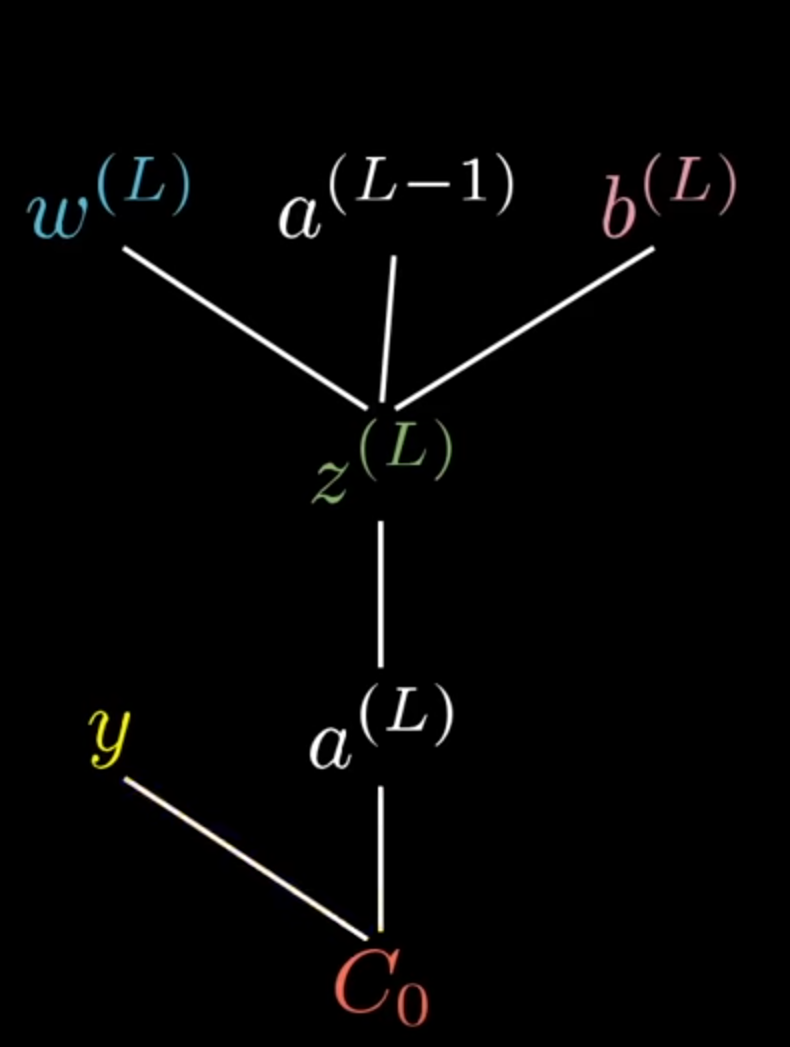
\includegraphics[width=0.8\textwidth]{images/3b1b_backpropagation.png}
    \caption{3B1B Backpropagation}
    \label{fig:Backpropagation}
\end{figure}

Ok lets first look at simple example and then expaldn it, lets say we only have 1 Neuron per layer now lets introduce some notations, as shown in the image. Lets focus on the connection of the last 2 Neurons first. $a^{L}$ being the activation of the last neuron, and $a^{(L-1)}$ being the activation of the previous neuron. So how do we determine the last activation well as we discussed it is determined by a weight $w^{(L)}$ the previous action $a^{(L-1)}$ and a bias $a=b^{(L)}$ and then an activation function. We also dicussed that we define a name for that here being $z^{(L)} = w^{(L)} \cdot a^{(L-1)} + b^{(L)}$ and $a^{(L)} = \sigma(z^{(L)})$. 
Now that we computed a as shown in the image we can compute the cost with a target value $y$ and a cost function $C$ This can be expanded to substituting the $a^{L-1}$ function as well of course. But lets focus on the last layer for now. The first thing that might be interesting here is how changes in the weight effect our cost function. In mathematical Terms we are 
interested in the derivative of the cost function with respect to the weight. $ \frac{\partial C_{0}}{\partial W^{(L)}}$ But how do we get there again with intuition the chain rule makes perfect sense here because what is important for that ratio to know. Well first $w^{(L)}$ effects $z^{(L)}$ which in turn effects $a^{(L)}$ which in turn effects the cost function. 
So lets write this down mathematically using the chain rule! 

\[
\frac{\partial C_{0}}{\partial W^{(L)}} = \underbrace{\frac{\partial z^{(L)}}{\partial w^{(L)}}}_{\shortstack{effect of \( w \) \\ with respect to \( z \)}} \underbrace{\frac{\partial a^{(L)}}{\partial z^{(L)}}}_{\shortstack{now that \( z \) changed \\ let's calculate the effect \\ that has on \( a \)}} \underbrace{\frac{\partial C_{0}}{\partial a^{(L)}}}_{\shortstack{effect of \( a \) \\ on the cost \( C_{0} \)}}
\]
Lets break down the terms now. So first the effect of a on the term C is just $2(a^{(L)} - y)$ The derivative of the activation function is just the derivative of the activation function. And the derivative of $z$ with respect to $w$ is just $a^{(L-1)}$. Because this relation just depends on ow strong the previous neuron was activated. Now this is just for a single training example if we wanted to compute this for 
all the Training examples we would compute an average meaning $$\frac{\partial C}{\partial W^{(L)}} = \frac{1}{n} \sum_{k = 0}^{n-1} \frac{\partial C_{k}}{\partial W^{(L)}}$$ Now we have succesfully computed one component of the gradient vector $C$ We would now need to do the same for the bias and the previous layers. For the bias the computation 
is almost the same, because we can just swap out every w for a b. But if we consider the derivative of $\frac{\partial z^{(L)}}{\partial b^{(L)}}$ we see that this is just 1. Because obviosuly a change in the Bias would result in a change of the activation exactly equivalent to the change in the Bias. Ok now lets look at how we go backward. The sensitivity of the cost function with respect to the activation of the last layer. In the formula it would look like this: \[ \frac{\partial C_{0}}{\partial a^{(L-1)}} = \frac{\partial z^{(L)}}{\partial a^{(L-1)}} \dots \] which in turn would just be the weight. Now since we kept track 
of this we can trace back how sensitive the cost function is to the activation of the previous layer. This is the basic idea of Backpropagation. Now this can be expanded to multiple neurons, however the Idea stays the same. One thing that changes is the cost function with respect to the activation of the previous layer. Lets introduce a new indeci to keep track which neuron talking about lets call it activation of the kth neuron in the L-1 layer with $a_k^{(L-1)}$ 
thus the cost function with respect to the activation of the kth neuron in the L-1 layer would be $\frac{\partial C_{0}}{\partial a_k^{(L-1)}}$ This can be computed by the chain rule as well, but we need to consider the entire layer L so we compute the sum which leads to the following equation $$ \frac{\partial C_{0}}{\partial a_k^{(L-1)}} = \sum_{j=0}^{n_{L}-1} \frac{\partial z_{j}^{(L)}}{\partial a_k^{(L-1)}} \frac{\partial a_j^{(L)}}{\partial z_j^{(L)}} \frac{\partial C_{0}}{\partial a_j^{(L)}}$$ 
I personally found the slides to be rather confusing that is why i mainly used 3B1B 4th video of his Neural Network Series to explain this.
\subsection{TODO explain this with jacobi matrices (i think before should work to understand the concept though)}

\section{Regularization}

\subsection{Gradient Clipping}

Sometimes Deep Neural Networks, have the  issue of exploding Gradients. This Problem occurs if Multiplying large weights. Visually this is explodingly steep parts in a Loss Function. The Problem is that with our current approach the Parameters of the Model would be updated by a large amount, making our previous progress in Optimizing useless. 
This is why we introduce Gradient Clipping. This is done by setting a Threshold for the Gradient. Here 2 Methods are common, the first one is to clip the Gradient if an Entry of the Gradient exeeds a certain Threshold, this is refered to as Value-Clipping. The second one would be Norm-Clipping if the Gradient exceeds a 
certain Norm, the Gradient is scaled down to the Threshold, this is refered to as Norm-Clipping.

\subsection{Parameter Initialization}

\subsubsection{Very Small Weights}
Lets talk about what happens with certain weights, starting with small weights. If the weights are too small, the Network might collaps to a linear Modell, which as previosuly discussed is not what we want. If we use the Sigmoid Activation Function and apply it to $W \cdot x$ with W being very small the Function becomes linear.

\begin{figure}[h]
    \centering
    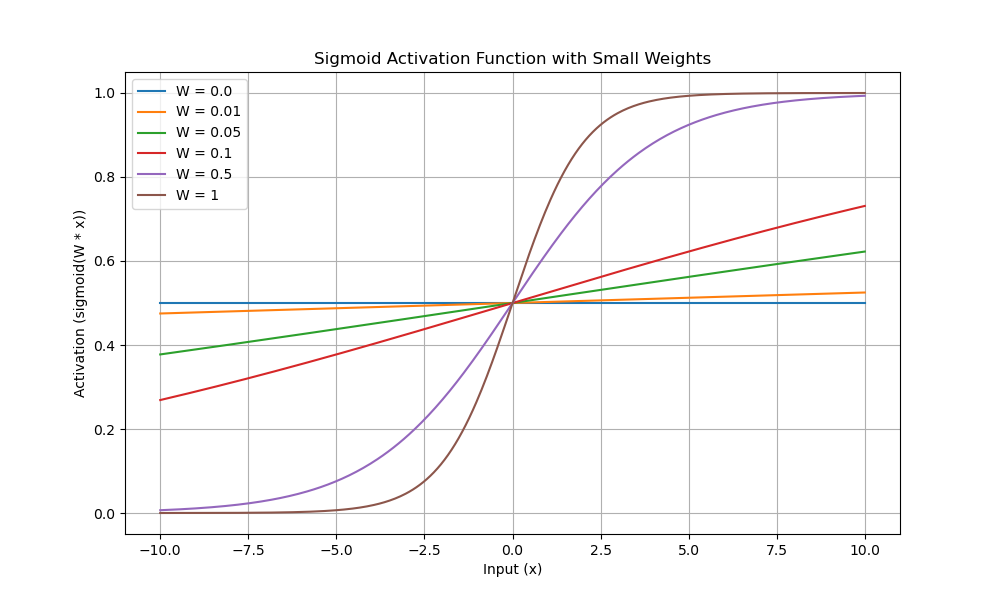
\includegraphics[width=0.8\textwidth]{images/sigmoid_small_weights.png}
    \label{fig:Sigmod Small weights}
\end{figure}
\newpage
\subsubsection{Very Large Weights}
Problems also arise with Very Large weights. With very large weights the Sigmoid Function becomes very steep, which makes the Gradient very small. This is a problem because the Gradient Descent would be very slow.

\begin{figure}[h]
    \centering
    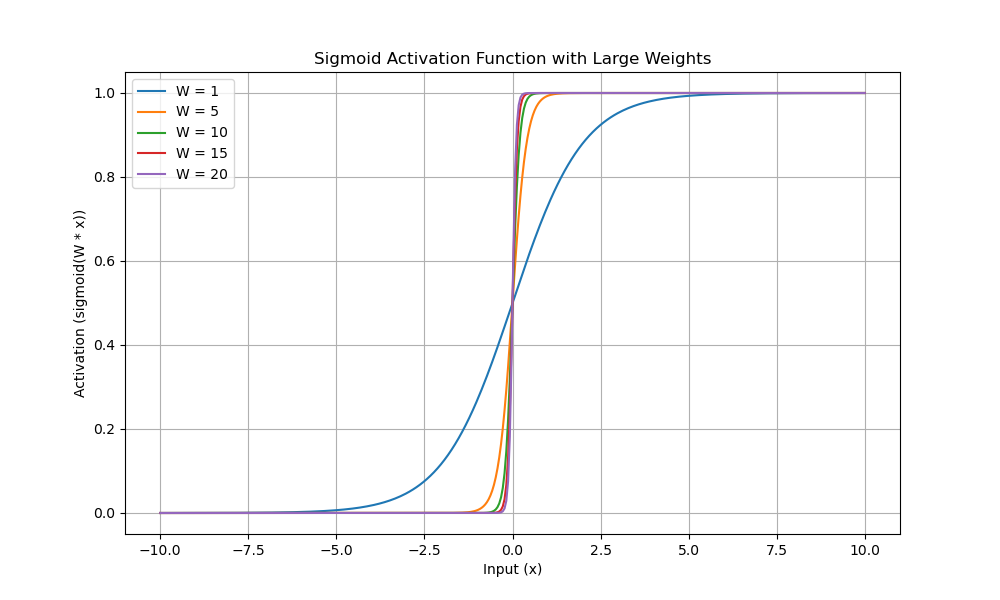
\includegraphics[width=0.8\textwidth]{images/sigmoid_large_weights.png}
    \caption{Sigmod with Large Weights}
    \label{fig:Sigmod Large weights}
\end{figure}

\subsection{Scalng the Input Values}
The range of Inputs determines the range of values for the Weights, thus making it important to scale the Input Values, because as we have seen this determines the quality of the Neural Net. A good rule of thumb is to scale the Inputs to have a mean of 0 and a standard deviation of 1. 
\subsection{Weight Initialization}
Usually the weights are initialized randomly with small values. So the network starts linear, but this will not remain the case when the weights are updated during training. Some might think it would make sense to initialize the weights with 0, but this would be problematic with the simplest reason being that 
the input for second layer would be the same for all Nodes, the output would be the same as well and would then be multiplied by the same weights. This would lead to the same output for all Nodes in the second layer, this goes on until the output layer, where it will still be zero.  Another reason would be that backpropagation would not
work, as the weights will be multiplied by a value determined by backpropagation but since the weights are zero they will remain zero, making our whole progress useless. 

\subsection{Parameter Initialization}
We want to initialize our parameter so that the Eigenvalues of the Jacobi Matrix and the Weights are close to 1. If the Eigenvalues are larger than 1, the Gradient will explode, if they are smaller than 1, the Gradient will vanish. This means that for the Jacobi Matrix of the actiavtion function with $J_{f^{(i)}}(a^{(i)})$ we want 
the derivative of the activation function to be close to 1. This is different from activation activation function to activation function though.  \\ 
\begin{itemize}
    \item Input Signals are usually scaled to have a mean of 0 and a standard deviation of 1. 
    \item Since the standard deviation of the output of a neuron is  1, the weights should be initialized and multiplied $\frac{1}{\sqrt{n}}$ with n being the number of inputs. This ensures ensures that the variance of the weighted sum remains 1, because the deviation of the weights is $\sigma^{2}$.
    \item The bias changes the mean of the output, usually it remains $0$ sometimes it makes sense to initialize it differently however. An example for that would be ReLU, where the bias should be initialized with a small positive value, so values lower than 0 are passed through the ReLU function.
\end{itemize}
\subsection{Scaling of the Weights as an Hyperparameter}
If we have enough computational power, we can use the scaling of the weights as a hyperparameter. This means that we can try different values for the scaling of the weights and see which one works best we can just experiment on Mini Batches though and check wether the Hidden Units are getting lower each layer. 

\subsection{Overfitting and Underfitting quick comeback in Context}
While Input and Output are usually fixed, the number of Hidden Units is a Capacity Parameter, we need to figure out. If we use too many neurons, the network will overfit, if we use too few neurons, the network will underfit. Deep Neural Networks are usually volotile to Overfitting, due to its high capacity. To prevent that Regularization 
is used.
\subsection{Definition of Regularization}
Regularization can be defined as any modification of a learning algorithm with the purpose of reducing the generalization error without significantly increasing the training error.
Common strategies to achieve this are adding more Terms to the Loss and Extra Constrains to the Modelparameters. Those strategies can use prior knowledge about the problem, but can also try to find a simple model for good generalization.
\subsection{Regularization in Deep Learning}
Most Regularization strategies want to find a good Bias Varianz Tradeoff. Which we have also talked about at the beginning. 

\subsection{Parameter Norm Penalties}
One way too force our Model to have a certain complexity is a so called Penality Term. This Term is added to the Loss Function. The Term is controlled by a Hyperparameter $\alpha$ and the Norm of the Parameters.   
\[
\tilde{L}(\theta; X, y) = \underbrace{L(\theta; X, y)}_{\text{Original Loss Function}} + \underbrace{\alpha \cdot \Omega(\theta)}_{\text{Penalty Term}}
\]

The Parameter Norm Penalty usually only applies to large Values in the weights, but not in the Biases, since the Bias only Influences a single Variable, meaning it needs little Data to be learned. If we would Introduce a Penalty Term for the Bias, underfitting becomes our Problem. 

\subsection{L2 Regularization}
A common and simple approach is the L2 Regularization. The L2 Regularization is defined as the sum of the squares of the weights. 
\[
\tilde{L}(\theta; X, y) = \underbrace{L(\theta; X, y)}_{\text{Original Loss Function}} + \underbrace{\alpha \frac{1}{2} ||w||^{2} }_{\text{L2 Norm Penalty Term}}
\]
This is also known as weight decay, because the weights are decaying to zero. In the Context of Backpropagation this means that the Gradient of the Penalty Term is added to the Gradient of the Loss Function. 
\subsubsection{TODO There is an intuition slide in the slides, which i cant explain well}
\subsection{L1 Regularization}
We have had the L2 Regularization, now lets talk about the L1 Regularization. The L1 Regularization is defined as the sum of the absolute values of the weights. For the loos function this means
The loss Function now is defined as:
\[
\tilde{L}(w; X, y) = L(w; X, y) + \alpha \cdot \|w\|_1
\]

and the Gradient:
\[
\nabla_w \tilde{L}(w; X, y) = \nabla_w L(w; X, y) + \alpha \cdot \text{sign}(w)
\]

\subsection{Sparse Networks}
The advantage of L1 Regularization is that it leads to sparse Networks. This means that the Network has many weights that are zero, so not Unit every unit in one layer is connected to every unit in another layer. This is useful because it saves computation time. 
\newpage
\subsection{Representation Sparsity}
\begin{figure}[h]
    \centering
    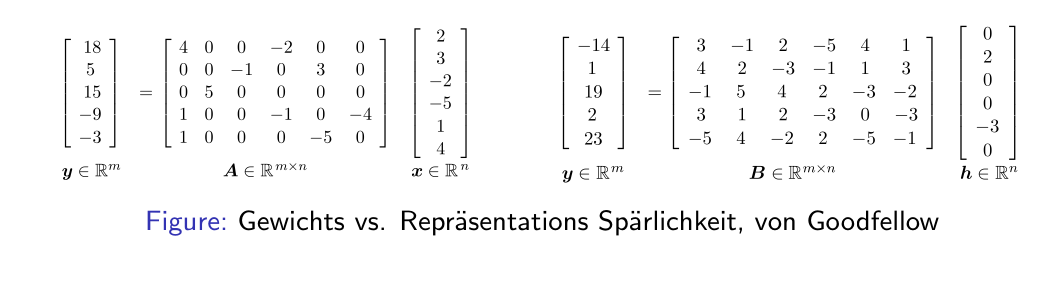
\includegraphics[width=0.99\textwidth]{images/sparsity.png}
    \caption{Different Sparsity}
    \label{fig:Sparsity}
\end{figure}
As visible in the figure in the Second way of writing the Vector the Vector multiply just forces Values to be sparse, since the Vector has Zero Values, while the weight Sparsity sets values of the Martix to $0$. 

\subsection{Regularization as Maximum A Posteriori Estimation}
The L1 and L2 Regularization can also be interpreted as Maximum A Posteriori Estimation. This means that we are looking for the most probable parameters given the data. The L2 Regularization can be interpreted as a Gaussian Prior, while the L1 Regularization can be interpreted as a Laplace Prior. This is not carried out in the slides, but I guess if you leave out the 
constant erm of the gaus prior we see that $\alpha$ is equivalent to $\frac{1}{2 \sigma^{2}}$. This surely works pretty similar for the Laplace distrubution.

\section{Reduction of Modelcapacity}
\subsection{Early Stopping}
One way to reduce the Modelcapacity is to stop the training early. This is done by monitoring the Validation Set and stopping the training when the Validation Error starts to increase. This is done because the Model is starting to overfit. The problem is that the Model might overfit faster, due to it recognizing patterns fast, it shouldnt have by training with the Validation Set.

\subsection{Exponential Moving Average}
We have learned about SGD already, here and issue might be the noise from the random selection of training data, this could lead to instable updating, therefore we introduce EMA which is defined as $$\theta_{EMA,t+1} = (1-\lambda) \theta_{EMA,t} + \lambda \theta_{t}$$ If $\lambda = 1$ then the EMA is just the parameter itself. If $\lambda = 0$ then the EMA is just the previous EMA. 

\subsection{Parameter Sharing}
In Regularization we assumed that we know, what the Model should look like, and thus can know which value will make sense and nudge the model in that direction, for example 0. This is not always the case, but sometimes we have knowldege the knowledge that for example two Models are close together. 
So lets say we have a Model A and a Model B with their respective parameters, we could apply a Parameter Penality, to force the Models to be similar, since we know they are. This would look like this $$ \Omega (\theta_{A}, \theta_{B}) = ||\theta_{A} - \theta_{B}||^{2}_{2} $$ 

We could also force the Parameters to be equivalent, which is done by Parameter Sharing. By Sharing parameters we essenstially tie weights together, meaning updates to the weights from one part of the Model will directly effect the others. If we think in text of Convolutional Neural Networks, we can think of the same filter being applied to different parts of the image. (This will be discussed later)

\subsection{Data Augmentation}
Data Augmentation is a technique to increase the size of the training set. This is done by applying transformations to the training data. (The one Python task from the practical Worksheet with the CIFAR Dataset)
\subsection{Injecting Noise}
Well we use Data Augmentation to make the Data a bit noisy so that the Neural Net is able to deal with Noise. We can also add Noice to hidden units. 
We can even add noice to the weights. 
\subsection{Noisy Outputs}
We can make the Outputs Noisy as well to make the Model robust to the Training Label being incorrect. This is done by saying our training label is just correct with a certain probability $1 - \epsilon$ 

\section{Bagging and Dropout}
\subsection{Bagging}
Bagging comes from the term Bootstrap Aggregating. This is basically the Introduction of Democracy. We train several models separately and then average the results, so every Model has the same vote in the final decision. This can be written as $$ p_{bagging} = \frac{1}{k} \sum_{i=1}^{k} p_{i}(y|x)$$ 

\subsection{Expected Error of Bagging}
If the test samples all do the same error, the expected error of the bagging is the same as the expected error of the single model. If the test samples do different errors, the expected error of the bagging is smaller than the expected error of the single model. 

\subsection{Creating the Models for Bagging}
The Models for Bagging are created by training the Model on different subsets of the training data. This is done by sampling the training data with replacement. This means that the same sample can be selected multiple times. This quite computationaly expensive, therefore we take a closer look at Dropout.
\subsection{Dropout}
Dropout is also to reduce complexity and overfitting, but it is an efficient way of performing Bagging, it just omits data during training. This is done by setting the output of a neuron to 0 with a certain probability. This is done for every neuron in the network. It just trains ensembles of all possible sub networks.(An ensemble refers to a combination of multiple models to solve a particular problem.) TODO why is this more efficient?

\subsection{Inference in Dropout}
First talk about how we calculate the Dropout. The Dropout $p_dropout$ is calculated by summing over all binary masks $\mu$ averaging over all possible sub networks, which can be formed by applying different binary masks. Now this is not computationally feasible, so we approximate this by randomly sampling binary masks, which turns out to be quite a good approximation. 
\subsubsection{Weight Scaling Inference Rule}
Ok so during Dropout we set the Neurons to zero with a certain Probabiliy $p$, as discussed before. But now we would like to use the entire Network, so we use something called Weight Scaling. During Inference we scale the Network Weights to $1-p$, this scaling accounts for the fact that during training we set the Neurons to zero with a certain probability.

\subsection{Bagging vs Dropout}
One major difference is that Bagging trains every model independently, while dropouts Subnetworks share Parameters, thus making it possible to compute even regarding the exponential number of possible Models. In Bagging every single Model is trained until converging this is not the case for Dropout. Due to the sheer Size of Dropout, we just train a fraction of the 
possible Models, then sharing is caring comes into play and we share the Parameters across the Models. All differences asside both methods are quite similar as Dropout Subnetworks can also be seen as Subsets of the original Network, which also are created when performing Bagging.

\subsection{Effectivity of Dropout}
Dropout is very effective in Regularization, and can be combined with other Regularization Techniques, we were Previosuly discussed. Dropout computes a Binary Mask per Training Sample in $O(n)$, and needs $O(n)$ Memory, to store the Binary Mask for Backpropagation. Weight Scaling is applied once for all Modelweights, thus making it Computationally irrelevant for Dropout. 
For Dropout it is important to note that we need large Models, since we reduce the Capacity of the Network by Dropout.

\subsection{Dropout in the Context of Noise Augmentation}
We used and learned about Augmentation, some might have noticed that Dropout adds Noise to the Network, as we loose out on some Information, and the Network is forced to learn with missing Information. 

\section{Basics of Convolutions}
NOTE: The following Introcution to Groups is brought to you by chatgpt and the slides as i am too lazy to Tex this. \\\\
Let \( G \) be a set and \( \cdot : G \times G \rightarrow G \) a binary operation. Then \((G, \cdot)\) is a group if:
\begin{enumerate}
    \item There exists an identity element \( e \in G \) such that \(\forall a \in G: e \cdot a = a \cdot e = a \).
    \item Every element \( a \in G \) has an inverse element \( a^{-1} \in G \) such that \( a \cdot a^{-1} = a^{-1} \cdot a = e \).
    \item Associativity holds: \(\forall a, b, c \in G : (a \cdot b) \cdot c = a \cdot (b \cdot c)\).
\end{enumerate}

\section*{Group Operation}

Let \((G, \cdot)\) be a group and \( X \) a set. Then \( \triangleright : G \times X \rightarrow X \) is a (left) group operation if:
\begin{enumerate}
    \item Identity: \(\forall x \in X : e \triangleright x = x\), where \( e \) is the identity element of \( G \).
    \item Compatibility: \(\forall a, b \in G, x \in X : (a \cdot b) \triangleright x = a \triangleright (b \triangleright x)\).
\end{enumerate}

\section*{Examples: Group Operations}

Transformations can be elegantly described using group operations. Let \( X = [0, 1]^{n \times n} \) be the space of images of size \( n \times n \).

\begin{enumerate}
    \item \( G = \{ \text{Id}, \text{Ref}_y \} \) forms a group containing the identity element (Id) and a reflection over the y-axis (Ref\(_y\)). That is, \(\text{Id} \triangleright x = x\) and \(\text{Ref}_y \triangleright x\) corresponds to the mirrored image of \( x \).
    \item \( G = \{ \text{Id}, \text{Rot}_{90}, \text{Rot}_{180}, \text{Rot}_{270} \} \) forms a group containing all 90° rotations of the image. What are the inverse elements of \(\text{Rot}_{90}\), \(\text{Rot}_{180}\), and \(\text{Rot}_{270}\)?
    \item \( G = \{ \text{Rot}_{\theta} : \theta \in \mathbb{R} \} \) forms a group containing all rotations. What problems could arise for a discrete and \( n \)-limited image space?
    \item \( G = \{ T(x, y) : x, y \in \mathbb{R} \} \) forms a group containing all translations by \( x, y \). What problems could arise for a discrete and \( n \)-limited image space?
    \item \( G = S(M) \) is the group of all permutations of a set \( M \). This group plays an important role, for example, in point cloud data.
\end{enumerate}

\section*{Equivariance and Invariance}

Let \( f : X \rightarrow Y \) be a mapping (for example, a neural network), \((G, \cdot)\) a group, and \(\triangleright : G \times X \rightarrow X\) and \(\square : G \times Y \rightarrow Y\) group operations on \( X \) and \( Y \) respectively.

\( f \) is called equivariant with respect to \( G \) if:
\[
\forall g \in G, x \in X : f(g \triangleright x) = g \square f(x)
\]

\( f \) is called invariant with respect to \( G \) if:
\[
\forall g \in G, x \in X : f(g \triangleright x) = f(x)
\]

\subsection{Convolution/Cross Correlation}
Ok now after the gpt Introduction to Groups, lets talk about Convolutions and Cross Correlations. 

For this I recommend the 3B1B Video on Convolutions, but lets try to explain it here as well. To quote the Video "The formulaic definition ... can look quite Intemidating".

But lets start slow and easy, imagine we have two lists of numbers (1,2,3) (4,5,6) and we can want to calculate the Convolution here. We would flip around list 2. So we would have (6,5,4) and then we would slide it over list 1. We would then multiply the corresponding elements and sum them up. So we have $(4 \cdot 1, 1 \cdot 5 + 2 \cdot 4, 1 \cdot 6 + 2 \cdot 5 + 3 \cdot 4, 
2 \cdot 6 + 3 \cdot 5, 3 \cdot 6) = (4, 13, 28, 27, 18)$. This is the Convolution of the two lists. Ok now lets look at the Formula.
The convolution of a function \( x(t) \) with a function \( y(t) \) is defined as:

\[
(x * y)(t) = \int_{-\infty}^{\infty} x(\tau) y(t - \tau) \, d\tau = \int_{-\infty}^{\infty} x(t - \tau) y(\tau) \, d\tau
\]
 
Now the $\tau $ is basicallty the flip to our list 2, just to give some intuition to the integral, considering our example the last equivalence in the definition makes sense as well, we could also reverse the first list and slide it over the second list, to achieve the same result. Here we can introduce the cross correlation, 
which is defined as: 
\[
(x \star y)(t) = \int_{-\infty}^{\infty} x(\tau) y(t + \tau) \, d\tau = \int_{-\infty}^{\infty} x(\tau  -t) y(\tau) \, d\tau = (x(- \tau ) * y(\tau))(t)
\]
This would be like multiplying the first list with the second list, but not flipping the second list, which would be the same as flipping the first list and sliding it over the second list. 
Ok lets visualize this with an example from the Slides. 
\begin{figure}[h]
    \centering
    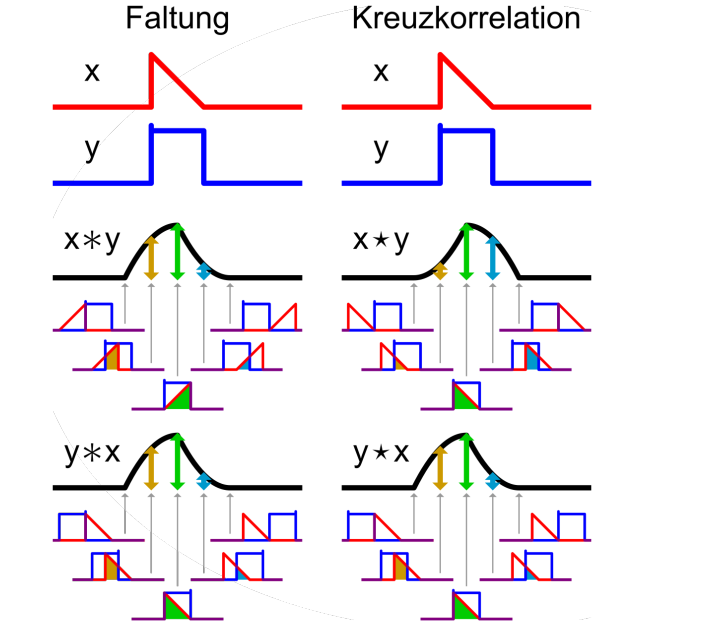
\includegraphics[width=0.8\textwidth]{images/convolution.png}
    \caption{Convolution}
    \label{fig:Convolution and Cross Correlation}
\end{figure}
Ok lets break down Convolution first, lets take the function y and flip like we have done to the list, and then we slide it over function x. Except the script image is explaining it with the second equivalence thus we flip x and slide it over y. The peak of the new function is basically in our example of the lists, where both lists are multiplied and added together. So imagine the first function coming closer to y and then we start multiplying
the corresponding components, so the value begins to increase and reaches its peak when both function overlap completly and then it decreases again. Lets have a closer look at the Slope of the Convolution here. The Slope is rather steep at the start and then decreases again, this is because the start of function y is steeper (imagine a larger number in the list)
decreasing it is not as steep, since the numbers are smalle for y. Now lets have a look at cross correlation, we just slide x over y, so the slope is not as steep at the start because the smaller part of x slides over y first. To put all of this into the two lists context, we can imagine the list y being (6,5,4) so the Bump at the start is our largest value at the start, try to think about this and watch the 3B1B Video. 
This example makes everyhting more intuitiv for me personally, how ever after reading this I do see if the explanation is a bit messy and all over the place, sorry for that.

\subsection*{Important Properties of  and Cross Correlation}

\begin{itemize}
    \item \textbf{Commutative:} \( x * y = y * x \)
    \item \textbf{Associative:} \( x * (y * z) = (x * y) * z \)
    \item \textbf{Distributive:} \( x * (y + z) = x * y + x * z \)
    \item \textbf{Convolution Theorem:} \( \mathcal{F}(x * y) = (2\pi)^{n/2} \mathcal{F}(x) \cdot \mathcal{F}(y) \), where
    \[
    \mathcal{F}(y)(f) = (2\pi)^{-n/2} \int_{\mathbb{R}^n} y(t) e^{-i f t} \, dt
    \]
    is the Fourier transform.
    \item Equivariant with respect to translations of \( x \) and \( y \).
\end{itemize}

\subsection*{Important Properties of Cross-Correlation}

\begin{itemize}
    \item \textbf{Distributive:} \( x \star (y + z) = x \star y + x \star z \)
    \item Equivariant with respect to translations of \( y \).
\end{itemize}
\subsection{Discrete Convolution/Cross Correlation}
With all my brambling about the lists, discrete Convolution should be rather intuitiv, we just sum up the products of the corresponding elements. The Discrete Convolution is defined as:
\[
(x * y)[n] = \sum_{k \in \mathbb{Z}^{n}} x[k] y[n - k] = \sum_{k \in \mathbb{Z}^{n}} x[n - k] y[k]  
\]
The Discrete Cross Correlation is defined as:
\[
(x \star y)[n] = \sum_{k \in \mathbb{Z}^{n}} x[k] y[n + k] = \sum_{k \in \mathbb{Z}^{n}} x[k-n] y[k]
\]

Here if you go over the list and stay within the bounds of the list that k provides, you are even good to go to see this as the formula from the first example. 

Ok but all of this kind of begs the question of why, why would we do that? In Visual Computing we often have images we refer here as a signal which is just a matrix of Pixel values(Probably a vector containing RGB or something), and we then want to apply a filter to the image this filter, which would be our function y is called a kernel. The Kernel is just a Small Matrix, which we slide over the image(yes like the 2 list of numbers) 
and then we apply the Convolution. (To get great visuals on this, i recommend the 3B1B Video on Convolutions). 
\newpage
\section{Convolutional Layers}
\subsection{Convolutional Layers in 1D}
We are going to use cross correlation now, lets say we have an Input Signal y, with the Kernel x(which is as mentioned before just a matrix) we are going to calculate the cross correlation $s = x \star y$. After calculating the cross correlation we apply an Activation Function to the result. This is the basic idea of a Convolutional Layer. It is also important to mention that we use weight sharing 
meaning we apply the same Kernels to every for example part of the image. This reduces the amount of Parameters when compared to fully connected layers. Also the connection are less, because we only apply our Kernels to a small part of the image.  This allows for the Sparsity discussed previously in connection to L1 Regularization.  An example of this can be seen in the following figure from the Slides.
\begin{figure}[h]
    \centering
    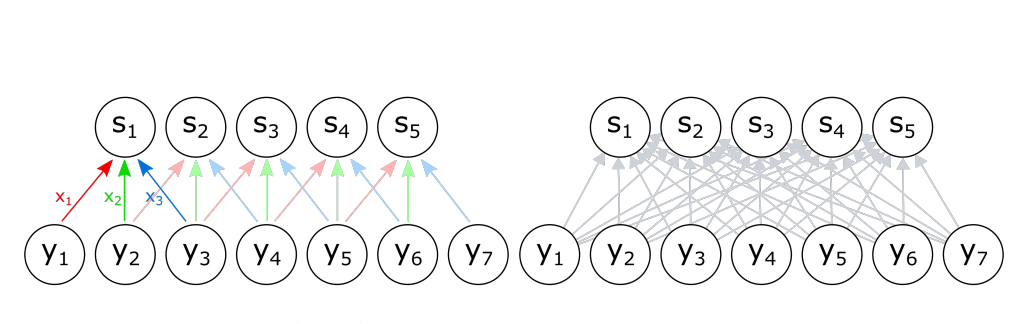
\includegraphics[width=0.8\textwidth]{images/convolutionalvsfullyconnected.png}
    \caption{Convolutional Layer}
    \label{fig:Convolutional Layer vs Fully Connected Layer}
\end{figure}
\subsection{Receptive Field}
Again considering images as signals, we can think of the Receptive Field as the part of the image that the Kernel is applied to. The Receptive Field is the area of the input image that has an effect on the output of the layer. This makes sense since the pixels in this case close to each other holds for other examples as well though are usually correlated 
and thus it makes sense to consider the once close to each other. This can also be seen in this figure from the slides.
\begin{figure}[h]
    \centering
    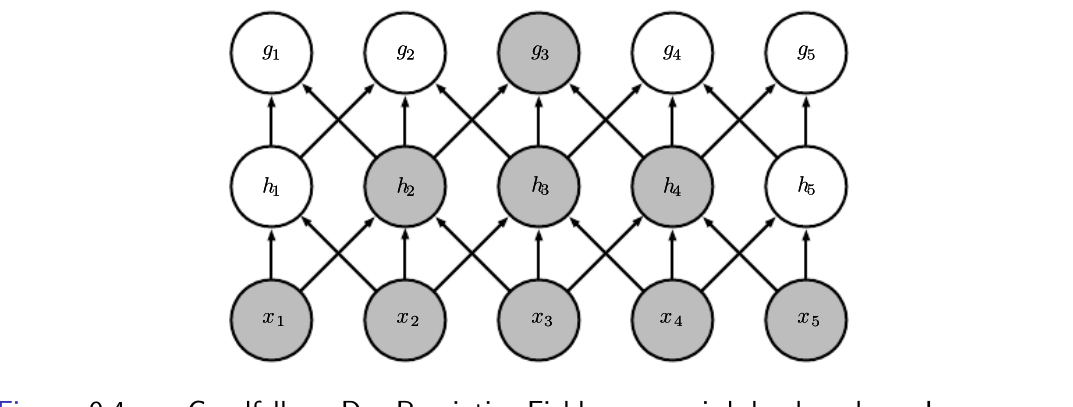
\includegraphics[width=0.8\textwidth]{images/receptive_field.png}
    \caption{Receptive Field}
    \label{fig:Receptive Field}
\end{figure}
Here g3 is effected by h2, h3, h4, which are in turn also always influenced by the previous layer. Which would be x1, x2, x3, x4, x5. This means the receptive field grows large in Multilayer Networks, even if the Kernel is small. 

\subsection{Dilation}
Another way to make the Receptive Field rather large is Dilation. Again in the context of pixels and images(imho the most intuitiv). In a traditional convolution, a filter slides over the input image, and at each position, it computes the dot product between the filter weights and the image pixels. The dilation introduces gaps between the filter weights. This means that the filter will skip over certain pixels in the input, effectively increasing the distance between the pixels it considers. This means that we can maybe get a broader context. 

\subsection{Padding}
Padding also makes sense lets again as always consider a Grid of Pixels, if we apply a Kernel of say size 3. If we apply the Kernel to the first Pixel of the image on a side we would loose that pixel, this would also happen if our Kernel reaches the last pixel of the image. This means that we would loose Every Pixel in the left pixel row, as well as the right, making our output smaller or less Dimensional. 
But this is not what we want we want to keep the Dimensionality of the Image, this is where Padding comes into play. Padding is just adding zeros around the image, so that the Kernel can be applied to every Pixel as we would basically just loose the zeros, instead of ours actual Pixels. This would then be called 0-Padding. There are also other types of Padding, such as Mirroring the Signal at the Edges or Peridodic Padding.(Not explained further on the slides, so I wont do it either.)

\subsection{Stride}
We can reduce the Dimensionality of the Output by using a Stride. The Stride is the amount by which the Kernel is moved over the Image. If we have a Stride of 2, the Kernel is moved by 2 Pixels. This also means that the Receptive Field Grows as our "context" grows larger. If we reduce Dimensionality it is also called Downsampling. 
\subsection{Pooling} 
In Pooling we can look at neighbouring Pixels and take an average or the maximum value. This also lets us assess context better, after we have done that we can for example do a stride operation again.
\newpage
\subsection{Example Max Pooling}
\begin{figure}[h]
    \centering
    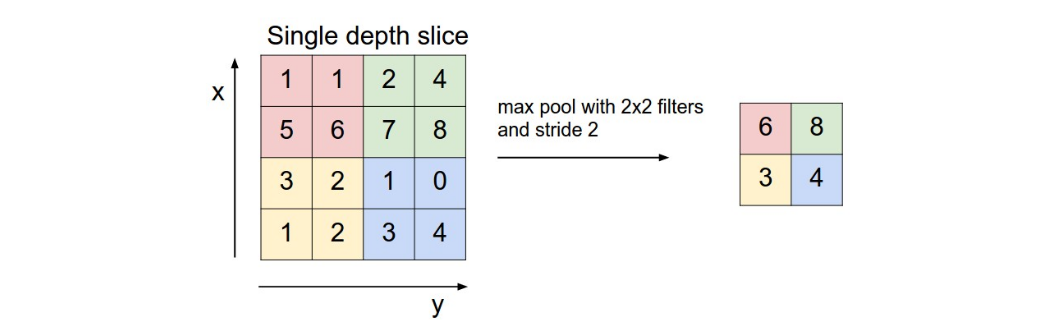
\includegraphics[width=0.8\textwidth]{images/maxpooling.png}
    \caption{Max Pooling}
    \label{fig:Max Pooling}
\end{figure}
This is an example of Max Pooling, here we just divide our image into 2x2 squares and take the maximum value of the 4 Pixels, since we use stride 2 there are no overlaps. This reduces the Dimensionality as can be seen in the output. 

\subsection{Convolutional Layers with Several Channels}
Ok this is where the Mind Fuck starts a bit. Lets talk about images. Our image has its set of pixels now and we always naively assumed the Pixels to have a certain value. But usually they might have multiple Values, for example RGB etc. This poses a Problem though, how we do we compute those with our Kernel Matrix. The answer is we dont we need a bit of a more sophisticated approach. 
So lets introduce 4 Dimensional Tensors. 

\begin{figure}
    \centering
    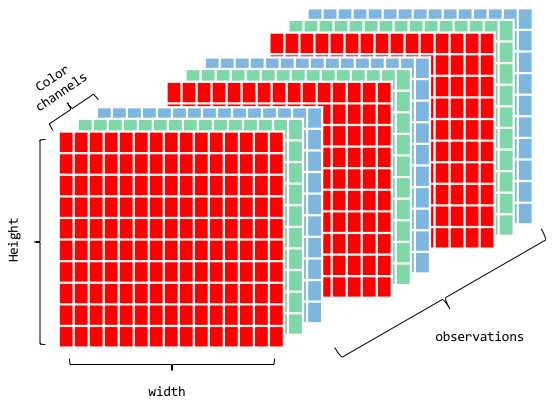
\includegraphics[width=0.5\textwidth]{images/4D_tensor.png}
    \caption{4D Tensor}
    \label{fig:4D Tensor}
\end{figure}
This figure depicts a 4D Tensor, lets break down what we need the Dimensions for, so first of all like before we need height and width of our Matrix. So we are in 2D Now, now all of those need to be applied to red green and blue, so now we are in 3D. Now we want to apply m filters for example to detect things such as  features like edges, textures, or colors, so for all of those we need different blocks of the 3D filters I just described. 
This is why we need the 4th Dimension. 

\subsection{Transpoed Convolution Layer}
This is the same process we have been discussing, for Convolution Layers, but in reverse. All the Concepts we learned can be applied to those as well in reverse. This is usefull for Decoders and Genrative Models.

\section{Batch Normalization}
We often have the issue that the input to the Activation Function is not centered around 0, this can lead to exploding or vanishing gradients. Now we learn about Batch Normalization in order to prevent that Problem. Batch Normalization can be applied to the Input but also the hidden layers. Ok if we take a look at the equation for Batch Normalization we see that we subtract the mean and divide by the standard deviation.
from a Matrix H which contains the activations for a Mini Batch. So $H' = \frac{H - \mu}{\sigma}$ So what does that do, well substracting the mean we center the activations around 0, and dividing by the standard deviation we scale the activations to have a standard deviation of 1. Forcing the activations to have a mean of 0 and a standard deviation of 1. It should be noted that the standard deviation also adds a really small number to prevent divison by 0. 

\subsection{Why is this usefull?}
If we consider activation Functions, such as the Sigmoid Function, if we input a very large number for exampe we get to a point where the function is almost flat, this means that the gradient is almost 0. This of course is problematic, thus normalizing makes perfect sense. In the Context of Inference, we need to keep track of a running average if the mean and standard deviation, 
so we can apply some kind of normalization to the test data.

\subsection{How we do it in Practice}
To my understanding this means that the Data might be more complex for us to adjust leave it normalized around zero, so we need to make it learn where it wants to be. This is done by introducing two new parameters, $\gamma$ and $\beta$. $\gamma$ is used to scale the normalized value and $\beta$ is used to shift the normalized value. Both of those are learned during training, we can always leave out the Bias, since $
\beta$ is pretty much the same but a bit more flexible. So now we calculate $\gamma \cdot H' + \beta$

\section{Convolutional Neural Networks Architectures}
TODO if someones to list them all here, too lazy for that, would be a bit of a prank if this comes in the exam.

\section{CNN visualization}
Probably makes more sense to read the slides, a lot of images. Would be weird to quizz on this, as it was never remotely part of the tasks or the practicals, as far as i can remember. 

\section{Transfer Learning}
We can do transfer learning if we for example have a classifier for cats, and now want to classify dogs. We cann use features of the cat network, to classify dogs. We could for example initialize the weights of the dog network with the weights of the cat network, this would probably give us a good starting point for gradient descent. 


\end{document}